\pagebreak

\chapter{Intermediate Code}\label{intermediatecode}

    The intermediate code produced by the 3PL compiler following immediate
    execution can be listed in file {\em design\_name}.icl by using option -t
    when calling 3PL. If option -pt is given instead the intermediate code
    prior to optimisation will also be listed. The listing will not include
    signal declarations (SIG elements - see below) but these can be included
    by using -T and -pT.

    The intermediate code consists largely of elements which can be
    expected to be available in any FPGA. This set of elements is enough
    to implement any 3PL program. Signals and signal arrays are arguments
    to these elements.
    
    The intermediate code list has undergone significant optimisation. Some
    additional optimisation occurs during low-level code generation
    (converting the intermediate code list into the output EDIF netlist).
    Additional logic minimisation occurs during later place-and-route by the
    FPGA vendor software.
    
    The intermediate code elements are -
    \blist
    \item   AND -       AND 2 or more signals
    \item   CONNECT -   connect a signal or signal array to another or to a
                        constant
    \item   CRAM -      a combinatorial-output RAM
    \item   DEL -       delay a signal one or more clock cycles
    \item   DFF -       a D-type flip-flop
    \item   DIVERGE -   handle queue divergence
    \item   DOWHILE -   a 'do while' statement
    \item   ELEMENT -   create a netlist element
    \item   EXECP -     delay execution on queue availability
    \item   IBUF -      an FPGA pad input buffer
    \item   ILOOP -     control an infinite loop
    \item   INV -       invert a signal
    \item   OBUF -      an FPGA pad output buffer
    \item   OPERATOR -  apply an expression operator to operands
    \item   OR -        OR 2 or more signals
    \item   PORT -      an external signal connection to/from another netlist
    \item   PRIORITY -  a priority encoder
    \item   QUEUEBUFFER - a queue variable (buffer)
    \item   REG -       a register
    \item   RESYNC -    resynchronise a pulse or edge to another clock
    \item   RRAM -      a registered-output RAM
    \item   SAMPLE -    sample a value in another clock domain
    \item   SELECT -    select one of several inputs
    \item   SIG -       declare a signal or signal array
 %   \item   SIMREAD -   read a value for a variable from a file during simulation
 %   \item   SIMWRITE -  write a value from a variable to a file during simulation
 %   \item   SIMVAR -    communicate program variables to the simulator
    \item   SPECIAL -   special functions for specific FPGA families
    \item   START -     start an execution stream
    \item   TSELECT -   a 3-state driver
    \item   WAIT -      wait for completion of parallel execution streams
    \item   WHEN -      a 'when' statement
    \item   WHILE -     a 'while' statement
    \item   XOR -       XOR 2 or more signals
    \blend
    

    \section{Signals}
    
        \subsection{variables}

            Global variables generate signals whose names begin with "glob.". Thus
            the output of a static global variable {\em a} would be a signal named
            {\em glob.a}.
            
            file module variables generate signals whose names begin with the
            file name, e.g. "prog.a".
            
            Modules, procedures and functions are nested within one of the file
            modules. A static variable {\em a} created within module {\em m}
            in file module prog
            would be signal "prog.m\_1.a" where an integer has been
            appended to distinguish variables created during different calls
            to the module. Further nested calls append more such strings
            to the identifier.
            
            Variables created within the scope of control structure blocks
            will have strings such as "if", "while" and "seq" appended to
            their signal identifiers.
            
            Signal array references have a subscript range appended, even
            if the entire variable is accessed, e.g. "glob.a[0..7]". For
            multiple ranges comma-separated ranges are shown, e.g.
            "glob.a[0..7,16..23]"

            \subsubsection{static variables}
            
                A global static variable {\em s} of size 8 bits would have
                the following associated signal arrays -
                \blist
                \item   "glob.s[8]" - the data output signal array
                \item   "glob.s.D[8]" - the data input signal array
                \item   "glob.s.CE[8]" - the clock enable signal array
                \item   "glob.s.RES[8]" - the set/reset signal array
                \blend                
                The value of the variable is available via the data output
                signal. Assignments are made by driving the data input
                signal and asserting the clock enable signals to the selected
                bits. The set/reset signal array is used to return some
                portion of the variable to its initial state.

            \subsubsection{queue variables}

                A global queue variable {\em p} of size 8 bits would have
                the following associated signal arrays -
                \blist
                \item   "glob.p[8]" - the data output signal array
                \item   "glob.p.D[8]" - the data input signal array
                \item   "glob.p.NE" - output availability (not empty)
                \item   "glob.p.POP" - pop a datum
                \item   "glob.p.PUSH" - push a datum
                \item   "glob.p.NF" - input availability (not full)
                \item   "glob.p.CNT[4]" - buffer occupancy count
                \item   "glob.p.SPC[4]" - buffer space count
                \item   "glob.p.RSTAT[5]" - buffer status in read clock domain
                \item   "glob.p.WSTAT[5]" - buffer status in write clock domain
                \blend
                These signals are further described in the section on queue
                buffers below.

            \subsubsection{value variables}

                Value variables are effectively pointers and can be assigned
                multiple times. To ensure that each assigned value is
                distinguished a unique integer is appended. A global value
                variable {\em v} of 8 bits might thus appear variously as
                "glob.v\_1", "glob.v\_2" etc.                 At the completion
                of immediate program execution the signal array "glob.v" would
                be equated with the last value the variable was assigned. This
                is an attempt to give the unappended variable identifier a
                sensible value during simulation (simulation is now disabled).

            \subsubsection{priority variables}

                A global priority variable {\em p} of size 8 bits would have
                the following associated signal arrays -
                \blist
                \item   "glob.p[8]" - the data output signal array
                \item   "glob.p.D[8]" - the data input signal array
                \item   "glob.p.PE" - the 'else' signal
                \blend


            \subsubsection{memory variables}

                Memory variables have separate signal array identifiers
                for each port, e.g. global combinatorial-output memory
                {\em m} with two ports would have port output signal arrays
                "glob.m\_0" and "glob.m\_1".


        \subsection{expressions and execution control signals}
        
            The values resulting from expressions are given signal array
            identifiers of the form "E9".
            
            Various other control signals are generated with prefices "A",
            "AND", "CD",, "CONST" "EO", "F", "FB", "FD", "FDCP", "FDRS", "FF",
            "FS", "I", "IN",, "INT" "INV", "LOG", "MADDR", "MDATA", "P", "PE",
            "PNTBUSY", "Q", "RADDR\_", "ROPAV", "S", "SAMPLEOUT", "SB", "SC",
            "SD", "SS", "start", "TF", "TS", "UINT" and "WADDR\_", integers
            being appended in each case to ensure identifiers are unique. There
            is no particular significance in these identifiers, the initial
            strings having been chosen to reflect the context in an attempt to
            improve readability of the intermediate code.


    \section{Intermediate code elements}


        \subsection{AND}

            \subsubsection{purpose}
            
                An AND gate for control signals.

            \subsubsection{arguments}
            
                \begin{tabular}{| l | l |}
                \hline
                Parameters  & none \\
                \hline
                Inputs      & input signal \\
                            & input signal \\
                            & . \\
                            & . \\
                \hline
                Outputs     & AND signal \\
                \hline
                \end{tabular}

            \subsubsection{description}
            
                AND two or more input signals, the result appearing on the
                output.

            \subsubsection{dump format}
            
                \begin{lstlisting}{gobble=16, language={tde}}
                       S11 = A12 & A14 & S8
                \end{lstlisting}

            \subsubsection{diagrammatic form}

                
\includegraphics{and}




        \subsection{CONNECT}

            \subsubsection{purpose}
            
                Connect signals or signal arrays.

            \subsubsection{arguments}
            
                \begin{tabular}{| l | l |}
                \hline
                Parameters  & optional boolean for cast sign extension \\
                \hline
                Inputs      & signal, signal array or constant \\
                \hline
                Outputs     & signal or signal array \\
                \hline
                \end{tabular}

            \subsubsection{description}
            
                This connects signals or signal arrays.
                
                If there is a single boolean parameter the operation is a cast.
                A true value indicates sign extension will be used if the output
                is wider than the input. A false value indicates zero padding
                will be used if the output is wider than the input. If the
                output is narrower than the input then truncation will occur and
                the parameter is not relevant. The parameter may be omitted or
                null.

                If there is no cast parameter and the input and output arrays
                are the same size then they will be simply connected.

                If there is no cast parameter and the input is a single bit
                then it will be connected to all outputs ('expand').

                If there is a cast parameter then the inputs will be connected
                to the outputs with possible size adjustment. If the output is
                smaller than the input then truncation will occur. If the
                output is larger than the input then the cast parameter will
                determine if sign extension (true 'cast - sign\_extend') or zero
                padding (false 'cast - pad') is used.
                
                If the input is a constnt TDEVar then the output signal array
                is connected to a pattern of GND and VCC to implement a 64-bit
                constant. The constant (which may be signed) will be truncated
                to fit the signal array. This case may include a sign extension
                parameter, but the parameter is not relevant since the constant
                is guaranteed to fit the output width, including the sign.

            \subsubsection{dump format}
            
                \begin{lstlisting}{gobble=16, language={tde}}
                       S11 = TS15
                       E1[0..7] = glob.a[8..15]
                       E2[0..2] = VCC expand
                       E3[0..7] = 17
                       E4[0..15] = glob.v[0..11] cast - pad
                       E5[0..15] = glob.v[0..11] cast - sign_extend
                \end{lstlisting}
                





        \subsection{CRAM}

            \subsubsection{purpose}
            
                Combinatorial-output RAM.

            \subsubsection{arguments}
            
                \begin{tabular}{| l | l |}
                \hline
                Parameters  & Integer number of ports \\
                            & Integer data width in bits \\
                            & Integer address width in bits \\
                            & String[] optional initialisation \\
                            & String - "tnm" attribute key \\
                            & String - data for "tnm" attribute \\
                \hline
                Inputs      & clock signal, port0 \\
                            & address array, port0 \\
                            & data\_in array, or null, port0 \\
                            & write signal, or null, port0 \\
                            & clock signal, port1 \\
                            & address array, port1 \\
                            & data\_in array, or null, port1 \\
                            & write signal, or null, port1 \\
                            & ..etc.. \\
                \hline
                Outputs     & data\_out array, or null, port0 \\
                            & data\_out array, or null, port1 \\
                \hline
                \end{tabular}

            \subsubsection{description}

                This is a RAM with a clocked write but a combinatorial read. At
                all times the output for a port reflects the memory contents at
                the location indicated by the current address input.

                The 2nd parameter gives the data width and the address width
                gives the memory depth (number of words). All port addresses
                must be the same width and all port data inputs and outputs must
                be the same width. The initialisation string array has one entry
                for each initial value. Each entry is a hexadecimal string. The
                initialisation array may be smaller than the depth of the RAM
                but not larger. The initialisation parameter may be omitted in
                which case the RAM is explicitly initialised to all 0. Ports
                which are not written have null arguments for the data in and
                the write enable. Ports which are not read have null arguments
                for the data out.

                For Xilinx FPGAs Combinatorial-output RAM is CLB RAM. The
                address width is limited to a maximum of 9 bits (a depth of 512
                words). The data width is not limited.
                    
                There is one optional attribute which is a timing group name.
            
            \subsubsection{dump format}
            
                \begin{lstlisting}{gobble=16, language={tde}}
                   CRAM - 2 ports {
                    OUT0	/Users/dun202/lib/3pl/3pl_lib/csiro/hymod/io2.trailermodule_0.ext_ram_trailer_0.forvar_7385.for_8025.if_8700.read_write_1.forvar_8782.for_8783.if_8784.pfifo_1.mem_0[0..35]
                    OUT1	/Users/dun202/lib/3pl/3pl_lib/csiro/hymod/io2.trailermodule_0.ext_ram_trailer_0.forvar_7385.for_8025.if_8700.read_write_1.forvar_8782.for_8783.if_8784.pfifo_1.mem_1[0..35]
                    <-
                    CLK0	glob.ext_ram_clk
                    ADDR0	MADDR36129[0..3]
                    DATA0	MDATA36130[0..35]
                    WE0	S36137
                    CLK1	null
                    ADDR1	MADDR36152[0..3]
                    DATA1	-
                    WE1	-
                   }
                \end{lstlisting}
                
                The presence of an initialisation argument is flagged
                but the values are not listed.

            \subsubsection{diagrammatic form}


                
\includegraphics{cram}

                



        \subsection{DEL}

            \subsubsection{purpose}
            
                To create a delay line to delay a signal one or more clock
                cycles. The input and output may be any width. The delay may be
                variable.

            \subsubsection{arguments}
            
                \begin{tabular}{| l | l |}
                \hline
                Parameters  & Integer number of clock cycles to delay if constant,
                              else 0 \\
                            & String array  initial words in line as array of hexadecimal strings \\
                \hline
                Inputs:     & clock signal \\
                            & input signal array \\
                            & delay signal array  number of clock cycles to delay if
                              variable, else null \\
                            & enable signal delay steps if high - null for
                              every cycle \\
                            & reset or null \\
                \hline
                Outputs     & output signal \\
                \hline
                \end{tabular}

            \subsubsection{description}
            
                If the reset is present then a fixed delay line will be created
                using flip-flops, in which case the variable length input must
                be null.
                
                If the variable length input is not null the delay line will
                use CLB shift registers and the reset input must be null.
                The delay length is limited to 16 or 32 depending on the
                FPGA.
            
                If the variable delay is used, this value selects the point
                in the delay line from which the output is taken. 0 selects
                the output of the 1st delay element and 15 the output of the
                16th delay element. Note that changing this value will result
                in data being skipped (decreasing) or repeated (increasing).

                If there is initialisation data the number of words will
                be equal to the delay line length.
                If there is no initialisation data these parameters will
                be omitted.
                
                The optional reset input returns the logic to its initial
                state.

            \subsubsection{dump format}
            
                \begin{lstlisting}{gobble=16, language={tde}}
                DEL E69[0..3] <- p.in[0..3] CLK glob.c166 delay 18 initialised
                \end{lstlisting}

            \subsubsection{diagrammatic form}

                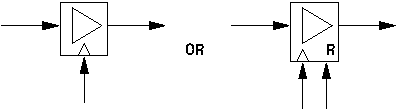
\includegraphics{del}



        \subsection{DFF}

            \subsubsection{purpose}
            
                A D-type flip-flop.

            \subsubsection{arguments}
            
                \begin{tabular}{| l | l |}
                \hline
                Parameters  & Boolean optional initial value \\
                            & integer type of flip-flop \\
                \hline
                Inputs      & data\_in signal, or null \\
                            & clock signal, or null \\
                            & clock enable signal, or null \\
                            & reset, set, clear or preset signal, or null \\
                \hline
                Outputs     & data\_out signal \\
                \hline
                \end{tabular}

            \subsubsection{description}

                This provides a basic D-type flip-flop. Unused arguments may be
                null and unused trailing arguments may be omitted.
                The 2nd argument specifies the type of flip-flop and the
                function of the 4th input signal-\\
                0 - FDRE - R (synchronous reset)\\
                1 - FDSE - S (synchronous set)\\
                2 - FDCE - CLR (asynchronous clear)\\
                3 - FDPE - PRE (asynchronous set)\\
                Any of the 1st (data in), 3rd (clock enable) or 4th
                (reset/set/clear/preset) signal inputs which are unconnectd
                will be connected to GND.
            
            \subsubsection{dump format}
            
                \begin{lstlisting}{gobble=16, language={tde}}
                   DFF {
                    OUT      FDRS622
                    <-
                    D        -
                    C        glob.ruclk
                    CE       -
                    R        OR621
                    S        S601
                   }
                \end{lstlisting}

            \subsubsection{diagrammatic form}

                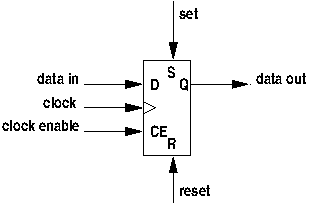
\includegraphics{dff}




        \subsection{DIVERGE}

            \subsubsection{purpose}
            
                A controller for divergent queue signals. Where a queue is read
                within more than one module it is required that each module
                execute a read before the datum is popped. Until all destination
                modules have executed a read the queue must appear unavailable
                for reading to those modules that have already executed a read.
                This is accomplished by inserting this DIVERGE element between
                the queue .NE and .POP signals and the .NE and .POp signals seen
                by the queue reads in each destination module.

            \subsubsection{arguments}
            
                \begin{tabular}{| l | l |}
                \hline
                Parameters  & none \\
                \hline
                Inputs      & clock signal \\
                            & reset signal \\
                            & queue not empty signal \\
                            & module queue pop signal \\
                            & module queue pop signal \\
                            & . \\
                            & . \\
                            & . \\
                \hline
                Outputs     & queue pop signal \\
                            & module queue not empty signal \\
                            & module queue not empty signal \\
                            & . \\
                            & . \\
                            & . \\
                \hline
                \end{tabular}

            \subsubsection{description}

                This splits the source queue .NE (read availability) and .POP
                (acknowledge) signals into a pair per destination module. The
                1st input is the output (read) clock signal for the queue.

                The 2nd input is the .NE (read availability) signal from the queue.
                The 1st output signal is the .POP (acknowledge) signal to the
                queue. The 2nd input is a reset which is asserted if the source
                queue is reset. The 3rd input is the .POP signal from the 1st
                module. The 2nd output is the .NE signal to the 1st module.
                Further input and output signals to other modules may follow. If
                there is only one module the .NE and .POP signals should be just
                connected through. If all destination acknowledge signals go
                high simultaneously the acknowledge signal to the source also
                goes high, otherwise it goes high when the last destination
                acknowledge signal goes high. The destination acknowledge signal
                is high for one clock cycle. When each destination acknowledge
                signal goes high the matching destination availability signal
                will go low at the next clock cycle unless all destination
                modules have also acknowledged in which case destination
                availability signals will be the be the same as the source
                availability signal.

            \subsubsection{dump format}
            
                \begin{lstlisting}{gobble=16, language={tde}}
                       DIVERGE {
                           in:
                               c100
                               S11
                               glob.p.NE
                               S21
                               S30
                           out:
                               glob.p.POP
                               S15
                               S22
                               S31
                       }
                \end{lstlisting}

            \subsubsection{diagrammatic form}

                
\includegraphics{diverge}

 

        \subsection{DOWHILE}

            \subsubsection{purpose}
            
                A {\em do while} statement.

            \subsubsection{arguments}
            
                \begin{tabular}{| l | l |}
                \hline
                Parameters  & none \\
                \hline
                Inputs      & start signal \\
                            & test signal \\
                            & block finish delayed signal \\
                            & optional reset signal or null \\
                            & clock signal \\
                            & optional reset signal or null \\
                \hline
                Outputs     & start signal for the body \\
                            & DO WHILE finish signal \\
                \hline
                \end{tabular}

            \subsubsection{description}

                The start input signal starts the first iteration of the loop by
                propagating straight through to the body start output signal. The
                block finish delayed input signal comes from the block finish
                signal, possibly via an EXECP if the test signal comes from an
                expression containing queue reads. The block finish delayed input
                signal is then routed either through to the body start output
                signal (test succeeds) or via a one cycle delay to the finish
                output signal (test fails).
                
                The optional reset signal clears internal state in the WHILE.

            \subsubsection{dump format}
            
                \begin{lstlisting}{gobble=16, language={tde}}
                   DO WHILE {
                       START_B     S23
                       FINISH      F35
                       <-
                       START       S24
                       TEST        E31[0]
                       CONTIN      F33
                       CLK         glob.c100
                       RESET       s34
                   }
                \end{lstlisting}

            \subsubsection{diagrammatic form}

                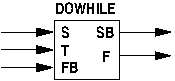
\includegraphics{dowhile}




        \subsection{ELEMENT}

            \subsubsection{purpose}
            
                Create an instance of a netlist element.
                
            \subsubsection{arguments}
            
                \begin{tabular}{| l | l |}
                \hline
                Parameters  & String  the element name               \\
                            & String  netlist block name or null     \\
                            & String    port name         | 1st port \\
                            & integer   port type         |          \\
                            & integer   port width        |          \\
                            & integer   port array format |          \\
                            .                             | 2nd port \\
                            .                                        \\
                \hline
                Inputs      & input 1                                \\
                Inputs      & input 2                                \\
                .                                                    \\
                .                                                    \\
                \hline
                Outputs     & output 1                               \\
                Outputs     & output 2                               \\
                .                                                    \\
                .                                                    \\
                \hline
                \end{tabular}

            \subsubsection{description}

                This is used to explicitly create a component element. It can be
                used to access library components which are not available
                implicitly in normal code or to access external elements such as
                cores. It is useful for accessing hardware elements which are
                peculiar to a particular FPGA rather than being generic.
                Examples of this are Xilinx global clock buffers as these are
                not generic elements normally generated implicitly by the
                compiler.

                The first parameter is the element name. The optional second
                parameter is a netlist identifier for this instance of the
                element. If null an arbitrary identifier of the form "b123" will
                be generated.
                
                The following parameters are quadruples giving the port name,
                port type (0 input, 1 output, 2 3-state output, 4 clock input),
                port width in bits and port array format, 0 for non-array
                ports, 1 for pins as A1, A2, A3 etc. and 2 for EDIF pin arrays.
                For each quadruple there will be an associated signal in the
                input or output list in the order of occurrence in the
                parameter list.
            
            \subsubsection{dump format}
            
                \begin{lstlisting}{gobble=16, language={tde}}
                   ELEMENT DCM block dcm1
                    PIN CLKIN I glob.ruclk
                    PIN CLKFB I prog.cfb
                    PIN CLK0  O prog.cfb_raw
                    PIN CLKDV O prog.pclk_raw
                \end{lstlisting}


        \subsection{EXECP}

            \subsubsection{purpose}
            
                An execution wait for queue availability and/or priority grant.

            \subsubsection{arguments}
            
                \begin{tabular}{| l | l |}
                \hline
                Parameters  & none \\
                \hline
                Inputs      & clock signal \\
                            & start signal \\
                            & buffered queue read/write availability signal \\
                            & unbuffered queue write availability signal \\
                            & unbuffered queue read availability signal \\
                            & priority output signal or null \\
                            & optional reset or null \\
                \hline
                Outputs     & delayed start signal \\
                            & priority input signal or null \\
                            & unbuffered queue write pending signal or null \\
                            & unbuffered queue read pending signal or null \\
                \hline
                \end{tabular}

            \subsubsection{description}
            
                This element delays an execution signal if it is necessary to
                wait for queue availability, for priority or both. The buffered
                queue availability input is high if all associated buffered
                queues to be read or written are available. The unbuffered queue
                availability inputs are similar but the write and read
                availabilities are on separate inputs.
                
                If the queue availability inputs are high and the priority
                encoder passes the signal, the execution signal is passed
                through without delay. If the queue availability inputs are not
                all high or priority has been pre-empted, the execution signal
                is stored until the queue availabilities are high and priority
                is granted at which time a single cycle output pulse is
                generated. An input execution signal must not occur when an
                output is pending however it may occur on the cycle following
                the output pulse. The queue availability inputs may be several
                queue availabilities ANDed together. The reset input, if not
                null, is used to clear any pending execution (waiting on queue
                availability or priority). The pending signals are used to
                notify unbuffered queues that a write or read is pending
                awaiting unbuffered queue availability. It is asserted when the
                start signal is asserted or the registered start signal is
                asserted and all buffered queues are available. The output need
                not have an argument (null) if unbuffered queues are not
                involved.

            \subsubsection{dump format}
            
                The dump format depends on which inputs and outputs
                are used.
            
                \begin{lstlisting}{gobble=16, language={tde}}
                   EXECP {
                        START_DEL SD250
                        PRI_IN    -
                        WPENDING  -
                        RPENDING  -
                        <-
                        CLK       glob.ruclk
                        START_IN  S262
                        BQAV      kandinski.link_0.if_3372.xc2vp_mgt16_0.q1.NF
                        UBQWAV    -
                        UBQRAV    -
                        PRI_OUT   -
                        RESET     -
                   }
                \end{lstlisting}

            \subsubsection{diagrammatic form}

                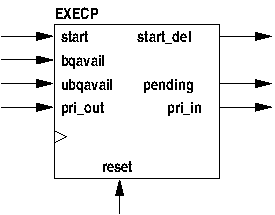
\includegraphics{execp}


            
        \subsection{IBUF}

            \subsubsection{purpose}
            
                A buffered external input signal.

            \subsubsection{arguments}
            
                \begin{tabular}{| l | l |}
                \hline
                Parameters  & String  - optional element identifier \\
                            & String  - input package pin \\
                            & String  - optional input package pin for differential input\\
                            & Boolean - ibufg flag \\
                            & Boolean - differential flag \\
                \hline
                Inputs      & input signal from pad \\
                            & optional differential input signal from pad or null \\
                \hline
                Outputs     & output signal \\
                            & optional differential output signal or null \\
                \hline
                \end{tabular}

            \subsubsection{description}

                This buffers an external input signal. The first parameter
                specifies the ID given to the IBUF element. The second parameter
                gives the primary FPGA pad designation. The third parameter is an
                optional second input pad for differential input or null. The
                fourth parameter is true for an IBUFG or IBUFGDS The last
                parameter is true if the input is differential (IBUFDS, IBUFGDS,
                IBUFDS\_DIFF\_OUT).
                
                There is a primary input signal followed by a second input
                signal if there is differential input to the IBUF
                (IBUFDS, IBUFGDS, IBUFDS\_DIFF\_OUT) or null (IBUF, IBUFG).
                
                There is a primary output signal followed by a second output
                signal if there is differential output from the IBUF
                (IBUFDS\_DIFF\_OUT) or null (IBUF, IBUFG, IBUFDS, IBUFGDS).
                
                There must be a {\bf loc} entry to specify the package pin. For
                differential inputs two consecutive pins are used, positive input
                followed by negative input.

            
            \subsubsection{dump format}
            
                \begin{lstlisting}{gobble=16, language={tde}}
                   IBUF    INPUT327[0] <- PORT_P88 loc=P88, IBUFG
                   IBUF    INPUT430[0] <- PORT_P91, PORT_P92 loc=P91,P92 IBUFDS
                \end{lstlisting}



        \subsection{ILOOP}

            \subsubsection{purpose}
            
                An infinite loop.

            \subsubsection{arguments}
            
                \begin{tabular}{| l | l |}
                \hline
                Parameters  & none \\
                \hline
                Inputs      & start signal \\
                            & block finish signal \\
                \hline
                Outputs     & block start signal \\
                \hline
                \end{tabular}

            \subsubsection{description}
            
                The start input signal is the start signal for all infinite
                loops in this clock domain. The block finish signal is high when
                the last statement in the code block executes. This element
                simply ORs the two inputs.

                Infinite loops containing a single statement that always
                executes in one clock cycle are replaced by a D-flip-flop which
                is set by the clock domain start signal and stays set thereafter
                since the contained statement is to execute on every clock
                cycle.

            \subsubsection{dump format}
            
                \begin{lstlisting}{gobble=16, language={tde}}
                       ILOOP       S12 <- glob.c100.start F14
                \end{lstlisting}

            \subsubsection{diagrammatic form}

                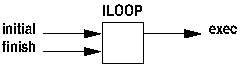
\includegraphics{iloop}






       \subsection{INV}

            \subsubsection{purpose}
            
                An single signal inverter.

            \subsubsection{arguments}
            
                \begin{tabular}{| l | l |}
                \hline
                Parameters  & none \\
                \hline
                Inputs      & input signal \\
                \hline
                Outputs     & output signal \\
                \hline
                \end{tabular}

            \subsubsection{description}
                
                The input and output are single signals, the output being the
                input inverted.

            \subsubsection{dump format}
            
                \begin{lstlisting}{gobble=16, language={tde}}
                       E17[1] = inv(glob.a[1])
                \end{lstlisting}

            \subsubsection{diagrammatic form}

                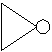
\includegraphics{inv}



        \subsection{OBUF}

            \subsubsection{purpose}
            
                A buffered external output signal.

            \subsubsection{arguments}
            
                \begin{tabular}{| l | l |}
                \hline
                Parameters  & String  - optional array of element identifiers \\
                            & String  - output package pin \\
                            & String  - optional output package pin for differential output\\
                            & boolean - differential flag \\
                \hline
                Inputs      & input signal \\
                            & optional 3-state enable signal (+ve for high-Z) or null\\
                \hline
                Outputs     & output signal to pad \\
                            & optional differential output signal to pad or null \\
                \hline
                \end{tabular}

            \subsubsection{description}

                This buffers an external output signal. The first parameter
                specifies the ID given to the OBUF element. The second parameter
                gives the primary FPGA pad designation. The third parameter is an
                optional second output pad for differential output or null. The
                fourth parameter flags a differential output.
                
                The first input signal is the data input. The second input signal
                is an optional 3-state enable which must be low to drive data onto
                the output pad (OBUFT, OBUFTDS). If this argument is null output
                drive to the pad is continuous (OBUF, OBUFDS).
                
                There is a primary output signal followed by a second output
                signal if there is differential output from the OBUF
                (OBUFDS, OBUFTDS) or null (OBUF, OBUFT).

                There must be a {\bf loc} entry to specify the package pin. For
                differential outputs two consecutive pins are used, positive output
                followed by negative output.

            \subsubsection{dump format}
            
                \begin{lstlisting}{gobble=16, language={tde}}
                   OBUF    PORT_P90 <- OUTPUTBIT213 loc=P90
                   OBUF    PORT_P92 <- OUTPUTBIT412 _EN=T31 loc=P92
                \end{lstlisting}


        \subsection{OPERATOR}

            \subsubsection{purpose}
            
                An arithmetic or logical operator.

            \subsubsection{arguments}
            
                The general form is

                \begin{tabular}{| l | l |}
                \hline
                Parameters  & enumerated type operator code \\
                Parameters  & enumerated type 1st operand type \\
                Parameters  & enumerated type 2nd operand type if binary or ternary \\
                Parameters  & enumerated type 3rd operand type if ternary \\
                Parameters  & enumerated type result type \\
                \hline
                Inputs      & 1st operand array \\
                            & 2nd operand array if binary or ternary \\
                            & 3rd operand array if ternary \\
                \hline
                Outputs     & output array \\
                \hline
                \end{tabular}

                The unused parameters and inputs are missing, not null.

            \subsubsection{description}
                
                Operator codes are -

                \begin{tabular}{| l | l |}
                \hline
                TDEOp.INV    & unary logical inversion \\
                TDEOp.NEG    & unary arithmetic negation \\
                TDEOp.ADD    & binary integer addition \\
                TDEOp.SUB    & binary integer subtraction \\
                TDEOp.ADDSUB & binary integer addition/subtraction \\
                TDEOp.MUL    & binary integer multiplication \\
                TDEOp.DIV    & binary integer division \\
                TDEOp.REM    & binary integer remainder \\
                TDEOp.DIVREM & binary integer division/remainder \\
                TDEOp.EQ     & binary equality test \\
                TDEOp.NE     & binary inequality test \\
                TDEOp.LT     & binary less-than test \\
                TDEOp.LE     & binary less-than-or-equal-to test \\
                TDEOp.GT     & binary greater-than test \\
                TDEOp.GE     & binary greater-than-or-equal-to test \\
                TDEOp.AND    & binary logical and \\
                TDEOp.OR     & binary logical or \\
                TDEOp.XOR    & binary logical exclusive or \\
                TDEOp.LSH    & binary left shift \\
                TDEOp.RSH    & binary right shift \\
                TDEOp.COND   & ternary conditional (\verb'?:') \\
                \hline
                \end{tabular}
                
                Arithmetic operations are either Ptype.UINT (unsigned integer)
                or Ptype.INT (signed integer). These may be mixed. If either
                operand is signed the result will be signed. The width of the
                result is that necessary to retain all significant bits.
                Operands to equality and inequality relational operators
                may be Ptype.UINT, Ptype.INT, Ptype.BITS or Ptype.LOG.
                Operands to the other four relational operators are
                Ptype.UINT or Ptype.INT. The first operand to the shift
                operators may be Ptype.UINT, Ptype.INT or Ptype.BITS. The
                second operand (shift count) must be Ptype.UINT. The shift count
                may be constant or variable. The ternary conditional operator
                first operator must be Ptype.LOG and the other two operands
                must be matching types (may be mixed Ptype.UINT and Ptype.INT)
                and types Ptype.UINT, Ptype.INT, Ptype.BITS or Ptype.LOG.
                
                The integer addition/subtraction operator provides conditional
                addition or subtraction by means of two additional input
                signals. The first selects addition (high) or subtraction (low).
                The second gates the second operand, high for add/subtract
                and low to inhibit add/subtract (output is first operand).
                This operation is available as an inbuilt function, not an
                operator.

                \begin{tabular}{| l | l |}
                \hline
                Parameters  & TDEOp.ADDSUB \\
                Parameters  & enumerated type 1st operand type \\
                Parameters  & enumerated type 2nd operand type \\
                Parameters  & enumerated type result type \\
                \hline
                Inputs      & 1st operand array \\
                            & 2nd operand array \\
                            & add/subtract control (high for add) \\
                            & pass 2nd operand control (2nd operand 0 if this is
                              low) \\
                \hline
                Outputs     & output array \\
                \hline
                \end{tabular}
                
                The integer division/remainder operator produces the quotient and
                remainder in a single division. For the division and remainder
                operators the quotient and remainder are both produced and
                one of these is discarded.
                This operation is available as an inbuilt procedure, not an
                operator.

            \subsubsection{arguments}
            
                \begin{tabular}{| l | l |}
                \hline
                Parameters  & TDEOp.DIVREM \\
                Parameters  & enumerated type 1st operand type \\
                Parameters  & enumerated type 2nd operand type \\
                Parameters  & enumerated type quotient type \\
                Parameters  & enumerated type remainder type \\
                \hline
                Inputs      & 1st operand array \\
                            & 2nd operand array \\
                \hline
                Outputs     & quotient output array \\
                Outputs     & remainder output array \\
                \hline
                \end{tabular}

            \subsubsection{dump format}
            
                \begin{lstlisting}{gobble=16, language={tde}}
                       OP E3[0..8] = E2[0..7] + glob.a[8..15]
                       OP E15[0] = !E14[0]
                       OP E20[0..7] = E4[0] ? blog.a[0..7] : E3[0..7]
                \end{lstlisting}

            \subsubsection{diagrammatic form}

                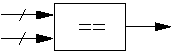
\includegraphics{op}
                
                Example of equality relational operator shown.


        \subsection{OR}

            \subsubsection{purpose}
            
                An OR gate for control signals.

            \subsubsection{arguments}
            
                \begin{tabular}{| l | l |}
                \hline
                Parameters  & none \\
                \hline
                Inputs      & input signal \\
                            & input signal \\
                            & . \\
                            & . \\
                \hline
                Outputs     & AND signal \\
                \hline
                \end{tabular}

            \subsubsection{description}
            
                OR two or more input signals, the result appearing on the
                output.

            \subsubsection{dump format}
            
                \begin{lstlisting}{gobble=16, language={tde}}
                       S11 = A12 | A14 | S8
                \end{lstlisting}

            \subsubsection{diagrammatic form}

                
\includegraphics{or}



        \subsection{PORT}

            \subsubsection{purpose}
            
                Flags a signal which is external to the current source code but
                is not external to the FPGA (i.e. not a pad connection). These
                signals are either connections to an imported core or are
                exported from the current source code which is itself a core.
                
            \subsubsection{arguments}
            
                \begin{tabular}{| l | l |}
                \hline
                Parameters  & Integer type of signal \\
                            & string  port name \\
                \hline
                Inputs      & signal or signal array \\
                \hline
                Outputs     & none \\
                \hline
                \end{tabular}

            \subsubsection{description}

                 The first parameter is an integer type code for the port type
                 which is 0 for input, 1 for output or 2 for 3-state output.
                 The second parameter is the port name.
            
            \subsubsection{dump format}
            
                \begin{lstlisting}{gobble=16, language={tde}}
                   PORT {
                       par:
                           Str     O
                           Int     ADDRESS
                       in:
                           Var     glob.addr[0..18]
                   }
                \end{lstlisting}



        \subsection{PRIORITY}

            \subsubsection{purpose}
            
                A priority encoder.

            \subsubsection{arguments}
            
                \begin{tabular}{| l | l |}
                \hline
                Parameters  & none \\
                \hline
                Inputs      & input signal 0 \\
                            & input signal 1 \\
                            & . \\
                            & . \\
                \hline
                Outputs     & output signal 0 \\
                            & output signal 1 \\
                            & . \\
                            & . \\
                \hline
                \end{tabular}

            \subsubsection{description}

            When one or more inputs are high the highest priority matching
            output signal will be high and all other outputs low. The inputs are
            ordered in decreasing priority (the 1st is highest).

            The number of outputs is equal to the number of inputs or the
            number of inputs + 1. In the latter case the last output is
            the 'else' case, i.e. no inputs high.

            \subsubsection{dump format}
            
                \begin{lstlisting}{gobble=16, language={tde}}
                   PRIORITY {
                    OUT   PRI_OUT40234[0,1,2,3,4]
                    ELSE  kandinski.processing_0.timer_0.mutex_var_0.pri.PE[0]
                    <-
                    IN    tPRI_IN40233[0,1,2,3,4]
                   }
                \end{lstlisting}

            \subsubsection{diagrammatic form}

                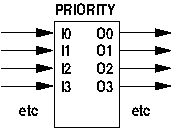
\includegraphics{priority}



        \subsection{QUEUEBUFFER}

            \subsubsection{purpose}
            
                A queue buffer.

            \subsubsection{arguments}
            
                \begin{tabular}{| l | l |}
                \hline
                Parameters  & Integer depth \\
                            & Boolean use hardware FIFO is possible, or null \\
                            & String initial value (hexadecimal string) or null \\
                \hline
                Inputs      & input clock signal, or null if same as output clock \\
                            & output clock signal \\
                            & input data array \\
                            & push datum signal (.PUSH) \\
                            & pop datum signal (.POP) \\
                            & reset signal (optional) \\
                \hline
                Outputs     & output data array                          \\
                            & read available signal (.NE - not empty)  \\
                            & write available signal (.NF - not full)    \\
                            & ready availability signal for unbuffered queue \\
                            & synchronous buffer occupancy count or null \\
                            & synchronous buffer space count or null     \\
                            & asynchronous buffer write status           \\
                            & asynchronous buffer read status            \\
                            & reset signal (optional) \\
                \hline
                \end{tabular}

            \subsubsection{description}

                A normal queue buffer has a depth of 2. If the depth is > 2, an
                initial value is not allowed. If a separate input clock is
                supplied, depths start at 16 and are various powers of 2
                depending on the size ranges of the block RAMs in the particular
                FPGA. If the input data array and output data array arguments
                are null then this is a null data queue buffer and the buffer
                depth is a power of 2 greater than 3.
                
                The 2nd output signal is the read availability signal. This is
                high if the buffered queue is not empty. For an unbuffered queue
                it is high if the queue is waiting on a write, i.e. it is
                connected to the PUSH input.
                
                The 3rd output signal is the write availability signal. This is
                high if the buffered queue is not full. For an unbuffered queue
                it is high if the queue is waiting on a read, i.e. it is
                connected to the POP input.
                
                The 4th output is null for a buffered queue. For an unbuffered
                queue it is the AND of the push (write) and pop (read) inputs
                (which is also the AND of the read availability (NE) and write
                availability (NF) signals.

                If the 5th output is not null this gives the number of words in
                a synchronous queue buffer synchronised to the queue clock (read
                and write).

                If the 6th output is not null this gives the number of free
                spaces in a synchronous queue buffer synchronised to the queue
                clock (read and write).

                If the 7th output is not null this gives the buffer status for
                an asynchronous queue buffer synchronised to the write (input)
                clock.

                If the 8th output is not null this gives the buffer status for
                an asynchronous queue buffer synchronised to the read (output)
                clock.

                If there is an 9th output this is a reset signal. This
                signal goes high for one clock cycle when the queuebuffer is
                reset via the reset() inbuilt procedure. For an asynchronous
                queuebuffer this signal is synchronised to the read (output)
                clock and is timed to follow the reset of the input (write)
                side of the queuebuffer.
            
                The asynchronous queue buffer status is a 5-bit word
                whose bits are -
                
                \begin{tabular}{| l | l |}
                \hline
                bit 0 & not full                        \\ \hline
                bit 1 & empty to 1/4 full + 1           \\ \hline
                bit 2 & 2 words to 1/2 full  + 1        \\ \hline
                bit 3 & 1/4 full + 1 to 3/4 full  + 1   \\ \hline
                bit 4 & 1/2 full + 1 to full            \\ \hline 
                bit 5 & 3/4 full + 1 to full            \\ \hline  
                \end{tabular}
                
                The bits are mutually exclusive and one of them is always set.
            
                Synchronous data queue buffers have a default depth of 2.
                Synchronous null queue buffers have a default depth of 16.
                Asynchronous data queue buffers have a default depth of 16.
                Asynchronous null queue buffers have a default depth of 16. Null
                queue buffers may have a depth which is 4 or greater and which is
                a power of 2. Data queue buffers may have the following depths -
                \blist
                \item   Spartan2, Virtex - 16, 256, 512, 1024, 2048 or 4096
                \item   Spartan3, Virtex2, Virtex2Pro, Virtex4 - 16, 512, 1024, 2048, 4096, 8192 or 16384
                \item   Virtex-5 - 64, 1024, 2048, 4096, 8192, 16384 or 32768
                \blend
                and for synchronous buffers depth 2 is also allowed and is
                the default.
                
                For queues of depth zero the signals have rather different
                meanings -
                \blist
                \item   PUSH - unbuffered queue write is pending from an EXECP
                \item   NE - connected to PUSH
                \item   POP - unbuffered queue read is pending from an EXECP
                \item   NF - connected to POP
                \blend
                outputs NE and NF simply reflect the PUSH and POP inputs. These
                are ANDed together to form an unbuffered queue availability
                signal (ready) back to the relevant EXECPs to synchronise the
                write/read pair.
                

            \subsubsection{dump format}
            
                \begin{lstlisting}{gobble=16, language={tde}}
                   QUEUEBUFFER  depth 2 {
                    OUT      kandinski.dps[0..11,12..21,22..30]
                    NE       kandinski.dps.NE
                    NF       kandinski.dps.NF
                    CNT      -
                    SPC      -
                    WSTAT    -
                    RSTAT    -
                    <-
                    CLKIN    -
                    CLKOUT   glob.ruclk
                    DATA     kandinski.dps.D[0..11,12..21,22..30]
                    PUSH     S5669
                    POP      SD5715
                    RESET    GND
                   }
                \end{lstlisting}
                
                The minimum size of the buffer is two and this is implemented as
                two registers. {\bf NF} stands for "Not Full", meaning
                that at least one free register is available for writing. {\bf
                PUSH} is ""push data onto queue". {\bf NE}
                stands for "Not Empty, meaning one or more registers contains
                data which can be read. {\bf POP} acknowledges a read, popping
                the word from the buffer (queue).
                
                Where a queue depth of zero is specified the "queue" is
                unbuffered. In that case this QUEUEBUFFER element simply
                connects OUT to DATA, NE to PUSH and NF to POP and there is no
                included logic. PUSH is now a write pending signal and POP
                a read pending signal. NE and NF are ANDed to form the unbuffered
                queue availability signal to both the read and write EXECP
                elements involved.

            \subsubsection{diagrammatic form}

                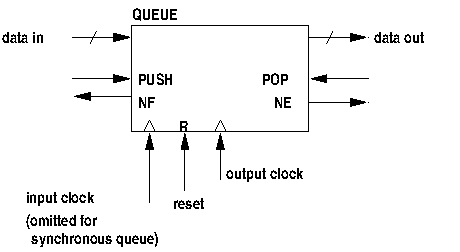
\includegraphics{queue}
                
                Buffer word and space counts and status outputs not shown.




        \subsection{REG}

            \subsubsection{purpose}
            
                A register (static variable).

            \subsubsection{arguments}
            
                \begin{tabular}{| l | l |}
                \hline
                Parameters  & String[] - block ids \\
                            & String - initial value \\
                            & boolean - IOB flag \\
                            & boolean - DSP flag \\
                \hline
                Inputs      & clock signal (may be null if .D null) \\
                            & data signal array (.D - may be null) \\
                            & clock enable signal or signal array (.CE) \\
                            & set/reset signal or signal array (.RES) \\
                \hline
                Outputs     & data signal array \\
                \hline
                \end{tabular}
                
                The block IDs are the identifiers for the DFF elements comprising
                the register, from LSB to MSB. The IOB flag indicates that the DFFs
                within I/O blocks should be used. This applies when the register
                input is connected to input buffers our its output is connected to
                output buffers. The DSP flag indicates that a DSP block may be used
                to implement the register instead of using CLB flip-flops.
                
                The either or both the clock enable and reset inputs may be
                single signals in which case they will be connected across all
                bits.

            \subsubsection{description}

                When the clock enable is high data will be clocked in on the next
                clock edge. For a primitive type all clock enable inputs are tied
                together as are all reset inputs. For a compound type clock enables
                and resets are grouped in words corresponding to primitives. The
                resets return the state to the initial value (0 by default). If the
                clock is null, there are no inputs to this register so generate a
                constant instead.


            \subsubsection{dump format}
            
                \begin{lstlisting}{gobble=16, language={tde}}
                       REG
                           OUT  glob.v[0..7]
                           <-
                           CLK  glob.c100
                           DATA glob.v.D[0..7]
                           CE   glob.v.CE[0..7]
                           R    glob.v.RES[0..7]
                           {0x0}{tnm=reg1}
                \end{lstlisting}
                The last line shows the initial value folowed by any flags.

            \subsubsection{diagrammatic form}

                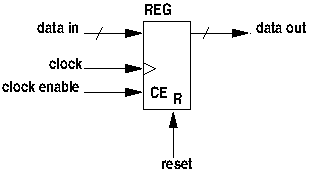
\includegraphics{reg}
                
                This only shows one word of a multiword register. Although
                they share a common identifier, the words of a register
                of compound type (array or struct) are independent. The data
                input and output will be labelled with the associated subscript
                range.


        \subsection{RESYNC}

            \subsubsection{purpose}
            
                A pulse or level resynchroniser.

            \subsubsection{arguments}
            
                \begin{tabular}{| l | l |}
                \hline
                Parameters  & none \\
                \hline
                Inputs      & input signal \\
                            & input clock signal \\
                            & output clock signal \\
                \hline
                Outputs     & output signal \\
                \hline
                \end{tabular}

            \subsubsection{description}

                The input may be a pulse or a level. When the input rises the
                rise is captured by the next input clock edge and an output
                pulse of one period duration is generated on the next output
                clock edge.

            \subsubsection{dump format}
            
                \begin{lstlisting}{gobble=16, language={tde}}
                   RESYNC {
                       in:
                           glob.a[0]
                           glob.c100
                           glob.bus_clk
                       out:
                           E41[0]
                   }
                \end{lstlisting}

            \subsubsection{diagrammatic form}

                
\includegraphics{resync}



        \subsection{RRAM}

            \subsubsection{purpose}
            
                Registered-output RAM.

            \subsubsection{arguments}
            
                \begin{tabular}{| l | l |}
                \hline
                Parameters  & Integer number of ports \\
                            & Integer data width in bits \\
                            & Integer address width in bits \\
                            & String[] optional initialisation or null \\
                            & String optional output register 0 string initial hex value, or null \\
                            & String optional output register 1 string initial hex value, or null \\
                            & String - attribute key \\
                            & String - data for attribute key \\
                            &       ...     other attribute pairs \\
                \hline
                Inputs      & clock signal, port0 \\
                            & address array, port0 \\
                            & data\_in array, or null, port0 \\
                            & read signal, or null, port0 \\
                            & write signal, or null, port0 \\
                            & clock signal, port1 \\
                            & address array, port1 \\
                            & data\_in array, or null, port1 \\
                            & read signal, or null, port1 \\
                            & write signal, or null, port1 \\
                            & ..etc.. \\
                \hline
                Outputs     & data\_out array, or null, port0 \\
                            & data\_out array, or null, port1 \\
                \hline
                \end{tabular}

            \subsubsection{description}

                This is a RAM with clocked read and write. The output for a port
                reflects the memory contents following a read clock cycle.

                The 2nd parameter gives the data width and the address width
                gives the memory depth (number of words). All port addresses
                must be the same width and all port data inputs and outputs must
                be the same width. The initialisation string array has one entry
                for each initial value. Each entry is a hexadecimal string. The
                initialisation array may be smaller than the depth of the RAM
                but not larger. The initialisation parameter may be omitted in
                which case the RAM is explicitly initialised to all 0. Ports
                which are not written have null arguments for the data in and
                the write enable. Ports which are not read have null arguments
                for the data out.

                For Xilinx FPGAs registered-output RAM is block RAM. The address
                width is limited to a maximum of 12 bits (a depth of 4096 words)
                for Spartan 2, Virtex and  Virtex E and 14 bits (a depth of
                16384 words) for Spartan 3, Virtex 2 and Virtex 2 PRO. The data
                width is not limited.
                
                Attributes are -
                \begin{tabular}{| l | l |}
                \hline
                loc             & block RAM location \\
                tnm             & timing group name \\
                writemode       & write mode \\
                writemodea      & port A write mode \\
                writemodeb      & port B write mode \\
                continuous      & continuous enable \\           
                \hline
                \end{tabular}
                There is one {\bf loc} attribute per block. Block RAM formats
                are selected by address width, then the number of blocks is
                determined by the total data width divided by the block data width.
                Block locations are in order from the least significant data bits.
                The other attributes are be applied to each
                individual RAMB4\_S, RAMB4\_S\_S, RAMB16\_S or
                RAMB16\_S\_S prepended in each case with "INST name "
                where 'name' is the generated netlist identifier for the
                RAM component.

            \subsubsection{dump format}
            
                \begin{lstlisting}{gobble=16, language={tde}}
                   RRAM - 2 ports {
                    OUT0	kandinski.link_0.if_3372.xc2vp_mgt16_0.crcunblock_0.buf_0[0..31,32]
                    OUT1	kandinski.link_0.if_3372.xc2vp_mgt16_0.crcunblock_0.buf_1[0..31,32]
                    <-
                    CLK0	glob.ruclk
                    ADDR0	MADDR1031[0..5]
                    DATA0	MDATA1032[0..31,32]
                    RE0	-
                    WE0	S1057
                    CLK1	glob.ruclk
                    ADDR1	S38113[0..5]
                    DATA1	-
                    RE1	S38114
                    WE1	-
                       initialised
                   }
                \end{lstlisting}
                
                The presence of an initialisation argument is flagged
                but the values are not listed.

            \subsubsection{diagrammatic form}

                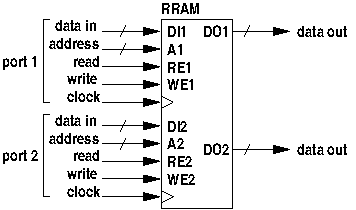
\includegraphics{rram}


        \subsection{SAMPLE}

            \subsubsection{purpose}
            
                Sample data from a different clock domain.

            \subsubsection{arguments}
            
                \begin{tabular}{| l | l |}
                \hline
                Parameters  & Boolean input clock freq > output clock freq \\
                \hline
                Inputs      & input data array \\
                            & input clock signal \\
                            & output clock signal \\
                \hline
                Outputs     & output data array \\
                \hline
                \end{tabular}

            \subsubsection{description}

                The input is sampled into the output clock domain. However, sampled
                data will not be corrupted depending on the relative
                clock rates data may be missed or multiply sampled. The input
                may be a different size to the output, zero padding or
                truncation being applied as required.

            \subsubsection{dump format}
            
                \begin{lstlisting}{gobble=16, language={tde}}
                   SAMPLE {
                       params:
                           true
                       in:
                           glob.a[0..7]
                           glob.c100
                           glob.bus_clk
                       out:
                           E41[0..7]
                   }
                \end{lstlisting}


        \subsection{SELECT}

            \subsubsection{purpose}
            
                Select one of several inputs.

            \subsubsection{arguments}
            
                \begin{tabular}{| l | l |}
                \hline
                Parameters  & String - unselected output value \\
                            & boolean - ALU flag \\
                            & boolean - DSP flag \\
                \hline
                Inputs      & select signal \\
                            & signal array \\
                            & select signal \\
                            & signal array \\
                            & . \\
                            & . \\
                            & . \\
                \hline
                Outputs     & signal array \\
                \hline
                \end{tabular}

            \subsubsection{description}

                The inputs are in pairs. The first of each pair is an
                input signal which selects the second of the pair (a signal
                array) to be connected to the output signal array. If no
                select signals are high the output is explicitly zero.
                The input arrays may be smaller than the output array.
                
                The data inputs may be narrower than the output in which case
                they will be padded or sign extended as appropriate.
                
                SELECT TDEs with only a single select/data input pair will be
                optimised away (data input connoected to output) unless the
                output is a queue variable which is not primitive. In that special
                case the SELECT TDE functions as a gate to ensure that a field
                or array member of a queue that is not explicitly assigned when
                the queue as a whole is assigned is assigned zero/false.

            \subsubsection{dump format}
            
                \begin{lstlisting}{gobble=16, language={tde}}
                       SELECT {
                           par:
                           in:
                               S11
                               glob.a[0..7]
                               S15
                               glob.b[24..31]
                           out:
                               glob.c[0..7]
                       }
                \end{lstlisting}

            \subsubsection{diagrammatic form}

                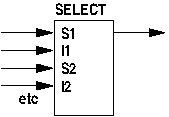
\includegraphics{select}


        \subsection{SIG}

            \subsubsection{purpose}
            
                Declare a signal or signal array.

            \subsubsection{arguments}
            
                \begin{tabular}{| l | l |}
                \hline
                Parameters  & none \\
                \hline
                Inputs      & signal or signal array \\
                            & signal or signal array \\
                            & . \\
                            & . \\
                \hline
                Outputs     & none \\
                \hline
                \end{tabular}

            \subsubsection{description}

                There may be any number of inputs. Each input
                may be a single signal or an array. Declarations
                are created which will be dimensioned if arrays.
                
                This element is only used by the simulator, not the code
                generator. It is not generated unless the -s or -T options
                are passed to the compiler.

            \subsubsection{dump format}
            
                \begin{lstlisting}{gobble=16, language={tde}}
                       SIG     glob.a
                       SIG     E1[1]
                       SIG     S11
                       SIG     mod1_1.a[8]
                \end{lstlisting}


%        \subsection{SIMREAD}
%
%            \subsubsection{purpose}
%            
%                Read a line from a file during simulation.
%
%            \subsubsection{arguments}
%            
%                \begin{tabular}{| l | l |}
%                \hline
%                Parameters  & string  file path name \\
%                \hline
%                Inputs      & clock signal \\
%                            & execution signal for the read \\
%                \hline
%                Outputs     & signal array driven from input data line \\
%                            & \ldots \\
%                            & \ldots \\
%                \hline
%                \end{tabular}
%
%            \subsubsection{description}
%
%                This element is only used by the simulator, not the code
%                generator. It is not generated unless the -s option
%                is passed to the compiler.
%                When the 2nd input signal is high, one line is read from the
%                file, is decoded according to the type of the output signal
%                arrays and the outputs are driven using the decoded values.
%                
%            
%            \subsubsection{dump format}
%            
%                This element is not printed.
%
%
%        \subsection{SIMWRITE}
%
%            \subsubsection{purpose}
%            
%                Write a line to a file during simulation.
%
%            \subsubsection{arguments}
%            
%                \begin{tabular}{| l | l |}
%                \hline
%                Parameters  & string  file path name \\
%                \hline
%                Inputs      & clock signal \\
%                            & execution signal for the write \\
%                            & signal array to be written to the data line \\
%                            & \ldots \\
%                            & \ldots \\
%                \hline
%                Outputs     & none \\
%                \hline
%                \end{tabular}
%
%            \subsubsection{description}
%
%                This element is only used by the simulator, not the code
%                generator. It is not generated unless the -s option
%                is passed to the compiler.
%                When the 2nd input signal is high, one line is written to the
%                file, each input signal array contributing one number to the
%                line.
%            
%            \subsubsection{dump format}
%            
%                This element is not printed.
%
%        \subsection{SIMVAR}
%
%            \subsubsection{purpose}
%            
%                A variable reference (only used by the simulator).
%
%            \subsubsection{arguments}
%            
%                \begin{tabular}{| l | l |}
%                \hline
%                Parameters  & Var class  variable \\
%                \hline
%                Inputs      & none \\
%                \hline
%                Outputs     & none \\
%                \hline
%                \end{tabular}
%
%            \subsubsection{description}
%
%                If the simulator is being used one of these elements is placed
%                on the list for every target variable.
%            
%            \subsubsection{dump format}
%            
%                This element is not printed.
%



        \subsection{SPECIAL}

            \subsubsection{purpose}
            
                Provides special functions, perhaps vendor specific.
                
            \subsubsection{arguments}
            
                \begin{tabular}{| l | l |}
                \hline
                Parameters  & Integer type of special function \\
                \hline
                Inputs      & \ldots \\
                \hline
                Outputs     & \ldots \\
                \hline
                \end{tabular}

            \subsubsection{description}

                 The first parameter is an integer type code which selects the
                 particular special function. At the moment there are only two
                 special functions.

                {\bf add line to the NCF or the XDC file}

                \begin{tabular}{| l | l |}
                \hline
                Parameters  & Integer 0 or 1 \\
                            & String  a format string \\
                \hline
                Inputs:     & signal  optional signal \\
                            & . \\
                            & . \\
                \hline
                Outputs:    & none \\
                \hline
                \end{tabular}

                The format string is written to the ISE NCF file or the Vivado
                XDC file. The format string may contain \%n or \%N conversions
                at which points netlist identifiers are to be inserted. The
                netlist identifiers are obtained from the input signals which
                are matched to the conversions in order. There will usually be
                at most one of these though the format allows any number. \%n is
                replaced by the identifier of the next input signal argument.
                \%N is similar to the above but changes the identifier to upper
                case and removes any leading "GLOB\_" string  This is used for
                generating clock timing group names from the clock signal
                identifier.

        \subsection{START}

            \subsubsection{purpose}
            
                Start an execution stream.

            \subsubsection{arguments}
            
                \begin{tabular}{| l | l |}
                \hline
                Parameters  & none \\
                \hline
                Inputs      & start level signal (may be VCC)\\
                            & domain clock signal \\
                \hline
                Outputs     & start pulse signal \\
                \hline
                \end{tabular}

            \subsubsection{description}

                The start input may be a pulse or a level. When the start signal
                rises the rise is captured by the next clock edge and an
                output pulse of one period duration is generated on the next
                clock edge. The logic is locked after this pulse so that
                any further start signal rises are ignored. The
                start level signal may be VCC if execution is to start
                immediately after configuration loading, otherwise it must be
                derived combinatorially from external inputs.

            \subsubsection{dump format}
            
                \begin{lstlisting}{gobble=16, language={tde}}
                   START { 
                    OUT  glob.uclk.start
                    <-
                    IN   VCC
                    COUT glob.uclk
                   }
                \end{lstlisting}

            \subsubsection{diagrammatic form}

                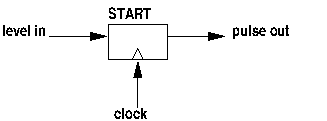
\includegraphics{start}


        \subsection{TSELECT}

            \subsubsection{purpose}
            
                A 3-state driver.

            \subsubsection{arguments}
            
                \begin{tabular}{| l | l |}
                \hline
                Parameters  & none \\
                \hline
                Inputs      & select signal \\
                            & signal array \\
                \hline
                Outputs     & signal array \\
                \hline
                \end{tabular}

            \subsubsection{description}

                The first of each input is a source signal array to be
                conditionally connected to the output signal array.
                The second input is an enable signal. When the enable is
                high the output is driven by the input. When the enable
                is low the output is not driven (is high impedance).
                The input array and output array must be the same size.

            \subsubsection{dump format}
            
                \begin{lstlisting}{gobble=16, language={tde}}
                       TSELECT {
                           par:
                           in:
                               glob.a[0..7]
                               S11
                           out:
                               glob.c[0..7]
                       }
                \end{lstlisting}


        \subsection{WAIT}

            \subsubsection{purpose}
            
                A parallel block completion wait.

            \subsubsection{arguments}
            
                \begin{tabular}{| l | l |}
                \hline
                Parameters  & none \\
                \hline
                Inputs      & clock signal \\
                            & reset signal or null \\
                            & input signal \\
                            & . \\
                            & . \\
                            & . \\
                \hline
                Outputs     & output signal \\
                \hline
                \end{tabular}

            \subsubsection{description}

                There are four or more inputs. The first input signal is the clock
                signal for the clock domain. The second input signal is a reset
                signal or is null if there is no reset. The third and following are
                finish signals. If all input signals go high simultaneously the
                output signal also goes high, otherwise the output signal goes high
                when the last input signal goes high. The output signal is high for
                one clock cycle. The reset input clears any pending latched
                completion signals.

            \subsubsection{dump format}
            
                \begin{lstlisting}{gobble=16, language={tde}}
                       WAIT {
                           in:
                               c100
                               null
                               S11
                               S13
                           out:
                               S15
                       }
                \end{lstlisting}

            \subsubsection{diagrammatic form}

                
\includegraphics{wait}


        \subsection{WHEN}

            \subsubsection{purpose}
            
                A {\em when} statement.

            \subsubsection{arguments}
            
                \begin{tabular}{| l | l |}
                \hline
                Parameters  & none \\
                \hline
                Inputs      & start signal \\
                            & test signal \\
                            & true block finish signal or null \\
                            & false block finish signal or null \\
                \hline
                Outputs     & true block start signal \\
                            & false block start signal \\
                            & WHEN finish signal or null \\
                \hline
                \end{tabular}

            \subsubsection{description}

                A start signal will be routed to either the true block start
                output or the false block start output according to whether the
                test input signal is high or low. The finish signals for the
                true and false blocks are returned as inputs and the OR of these
                emerges as the third output, signalling the end of the
                statement.

                A missing true or false block will have the block start signal
                connected back to the associated block finish signal via a
                1-cycle delay (TDEType.DEL). If both the true block and the
                false block require a single DEL for their finish signals these
                will be optimised to a separate common DEL from the start signal
                to the finish signal. In that case -
                \blist
                \item   true block finish signal
                \item   false block finish signal
                \item   WHEN finish signal
                \blend
                arguments to the WHEN will all be null.

            \subsubsection{dump format}
            
                \begin{lstlisting}{gobble=16, language={tde}}
                   WHEN {
                    T_START  S307
                    F_START  FS270
                    FINISH   F268
                    <-
                    START    S267
                    TEST     E274[0]
                    T_FINISH F281
                    F_FINISH FF312
                   }
                \end{lstlisting}

            \subsubsection{diagrammatic form}

                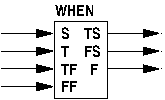
\includegraphics{when}

        \subsection{WHILE}

            \subsubsection{purpose}
            
                A {\em while} statement.

            \subsubsection{arguments}
            
                \begin{tabular}{| l | l |}
                \hline
                Parameters  & none \\
                \hline
                Inputs      & start signal \\
                            & test signal \\
                            & continuation signal from the body \\
                            & clock signal \\
                            & optional reset signal or null \\
                \hline
                Outputs     & start signal for the body \\
                            & WHILE finish signal \\
                \hline
                \end{tabular}

            \subsubsection{description}
            
            If the test input signal is high when start input signal goes high,
            the latter is routed to the body start output signal to execute the
            contained code block. If the test input signal is low when start
            input signal goes high, the latter is delayed by one clock cycle and
            then appears on the finish output signal (i.e. a {\em while} takes a
            minimum of one clock cycle). When the body code block finishes the
            last execution signal comes back to the continuation input signal.
            If the test input signal is high the continuation input signal is
            routed to the body start output signal to again execute the
            contained code block. If the test input signal is low the
            continuation input signal is routed through to the finish output
            signal, again with one clock cycle delay.

            The start signal and the continuation signal may come from
            EXECP elements which wait on queue availability in the test value.
                
            The optional reset signal clears internal state in the WHILE.

            \subsubsection{dump format}
            
                \begin{lstlisting}{gobble=16, language={tde}}
                   WHILE {
                    START_B    S505
                    FINISH     S516
                    <-
                    START      S502
                    TEST       E504[0]
                    CONTIN     F507
                    C          glob.ruclk
                    RESET      null
                   }
                \end{lstlisting}

            \subsubsection{diagrammatic form}

                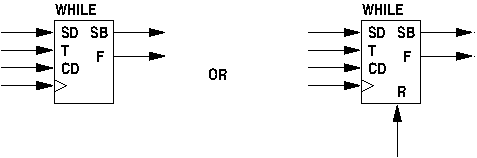
\includegraphics{while}


        \subsection{XOR}

            \subsubsection{purpose}
            
                An XOR gate for control signals.

            \subsubsection{arguments}
            
                \begin{tabular}{| l | l |}
                \hline
                Parameters  & none \\
                \hline
                Inputs      & input signal \\
                            & input signal \\
                            & . \\
                            & . \\
                \hline
                Outputs     & AND signal \\
                \hline
                \end{tabular}

            \subsubsection{description}
            
                Exclusive OR two or more input signals, the result appearing
                on the output.

            \subsubsection{dump format}
            
                \begin{lstlisting}{gobble=16, language={tde}}
                       S11 = A12 ^ A14 ^ S8
                \end{lstlisting}

            \subsubsection{diagrammatic form}

                
\includegraphics{xor}










    \section{Intermediate code optimisation}
        
        The intermediate code list is optimised by repeated applications of
        the following -
        \blist
        \item   Combine any {\bf EXECP}s with a common start and identical avail
                signal.
        \item   Combine any parallel {\bf DEL}s with a common start
                driving a common {\bf WAIT}.
        \item   Eliminate any {\bf DEL} in parallel with one or more EXECPs with
                a common start driving a common WAIT.
        \item   Eliminate any {\bf WAIT} that has a single input.
        \item   Eliminate any duplicate {\bf SELECT} inputs.
        \item   Find any AND or OR gates which have duplicated inputs
                and remove the duplicates. If this results in a single
                input remaining, eliminate the gate and connect
                the input to the output.
        \item   Find any {\bf INV}s with GND or VCC input and eliminate
                them, connecting the output to the inverse of the constant
                input.
        \item   Find any nested {\bf AND}, {\bf OR} or {\bf XOR} gates and
                consolidate them.
        \item   Find any control (not source code) {\bf AND} or {\bf OR} gates
                whose outputs are not connected and eliminate them.
        \item   Find any {\bf DEL}s whose outputs are not connected and
                eliminate them.
        \item   Find any WHENs which have a single {\bf DEL} in both the true
                block and the false block. Remove these and instead connect a
                single DEL from the start input to both the true block finish
                input and the false block finish input. This will result in
                an OR with identical inputs which will be eliminated by
                another optimisation iteration.
        \item   Eliminate any {\bf ILOOP}s which have the same output start
                signal and input finish signal. These infinite loops are
                empty, probably because they contain only value equivalence
                statements.
        \item   Find any {\bf ILOOP}s which have a single {\bf DEL} from the
                output start signal to the input finish signal. Replace the
                pair with a DFF whose SET input is driven by the start signal.
        \item   Find multiple {\bf DFF}s driven by a common {\bf START} and
                eliminate all but one.
        \item   Find any branch statements in which all branches, including
                the default, have a single DEL. Remove all the DELs and the
                final associated OR and replace with a single DEL from the
                start signal.
        \blend
        These optimisations are repeatedly applied to the list until a pass
        makes no change.


    \section{Intermediate code examples}

        % set frames for all further listings
        \lstset{
            basicstyle=\footnotesize\ttfamily,
            basewidth={0.5em},
            frame=single
        }
    
        Note that in the following examples the intermediate code dumps and the
        associated diagrams only show sections of the logic that illustrate the
        points under discussion - they are not complete listings or diagrams.
        
        In many cases clock inputs are not shown. The examples are constructed
        to use clock {\bf c100} and this can be assumed unless shown otherwise.
        
        In all the examples the signal {\bf glob.c100.start} appears. This is
        a single cycle pulse, synchronised to the {\bf c100} 100MHz clock, which
        is distributes to all execution threads to initiate them. In practice
        a recent change to the compiler has inserted a single cycle delay
        between this signal and every thread that it initiates but this is not
        shown in the examples. The purpose of the extra cycle is simply to avoid
        the path delays associated with distributing {\bf glob.c100.start} which
        can have a very high fanout. The inserted flip-flop in the path to each
        thread will be placed close the the logic that it initiates resulting
        in a much shorter path into the thread. {\bf glob.c100.start} will still
        have a high fanout but there is no combinatorial logic between its
        source and the myriad destination flip-flops.
    
        \subsection{top level sequential block}

            The code -
            \begin{lstlisting}[gobble=12, language=threepl]
               module "csiro/hymod/io1.3pl"

               useclock(c100);

               static({s1, s2}, "uint:8");

               seq {
                   s1 <- s2;
                   s2 <- s1;
               }
            \end{lstlisting}
            contains one execution thread. That thread will be an infinite loop
            containing two executable statements. The assignments do not wait on
            queues. The intermediate code would look like -
            \begin{lstlisting}{gobble=12, language={tde}}
               DEL F14 <- (1) glob.c100 S13
               DEL F17 <- (1) glob.c100 F14
               ILOOP       S13 <- glob.c100.start F17
               START       glob.c100.start <- START=VCC, CLK=glob.c100
               glob.s1.CE[0..7] = S13
               glob.s1.D[0..7] = glob.s2[0..7]
               glob.s1.RES[0..7] = GND
               REG
                   OUT  glob.s1[0..7]
                   <-
                   CLK  glob.c100
                   DATA glob.s1.D[0..7]
                   CE   glob.s1.CE[0..7]
                   R    glob.s1.RES[0..7]
                   {0x00}
               glob.s2.CE[0..7] = F14
               glob.s2.D[0..7] = glob.s1[0..7]
               glob.s2.RES[0..7] = GND
               REG
                   OUT  glob.s2[0..7]
                   <-
                   CLK  glob.c100
                   DATA glob.s2.D[0..7]
                   CE   glob.s2.CE[0..7]
                   R    glob.s2.RES[0..7]
                   {0x00}
            \end{lstlisting}
            The multiple versions of value variable {\bf start} (created
            in header code csiro/hymod/io1.3pl) are a result of the internal
            intricacies of the compiler. The last value the variable contains
            is assigned to the unappended identifier {\bf glob.start}
            in an attempt to provide a useful value in simulation (no longer
            enabled).

            Diagrammatically this is -

            
\includegraphics{e1}
            
            The thread is started from signal {\bf VCC} so element START generates
            a single pulse using clock {\bf c100}. This is injected into
            {\bf ILOOP} to start the infinite loop. The execution signal for the
            body of the infinite loop is {\bf S13}. The loop body is a {\bf seq}
            block containing two statements. The first is executed by {\bf S13} and
            a finish signal is generated one clock cycle later ({\bf F14}. This
            finish signal is the start signal for the next statement. A finish
            signal is generated one clock cycle later for the second statement
            ({\bf F17}). This second finish signal marks the completion of the loop
            body code so it is fed back to the {\bf ILOOP} to generate the next
            iteration. There is no delay in {\bf ILOOP} (it is simply an OR gate)
            so the loop executes every two clock cycles.

            The two execute signals, {\bf S13} and {\bf F14} control the
            assignments to the two static variables {\bf s1} and {\bf s2} via their
            CE inputs.

        \subsection{top level static assignment}
        
            If we simplify the above code so that the infinite loop contains
            only a single assignment -
            \begin{lstlisting}[gobble=12, language=threepl]
               static({s1, s2}, "uint:8");

               s1 <- s2;
            \end{lstlisting}
            then the intermediate code is -
            \begin{lstlisting}{gobble=12, language={tde}}
               START       glob.c100.start <- START=VCC, CLK=glob.c100
               glob.s1.CE[0..7] = S11
               glob.s1.D[0..7] = glob.s2[0..7]
               glob.s1.RES[0..7] = GND
               REG
                   OUT  glob.s1[0..7]
                   <-
                   CLK  glob.c100
                   DATA glob.s1.D[0..7]
                   CE   glob.s1.CE[0..7]
                   R    glob.s1.RES[0..7]
                   {0x00}
               glob.s2.RES[0..7] = GND
               REG
                   OUT  glob.s2[0..7]
                   <-
                   CLK  null
                   DATA null
                   CE   null
                   R    glob.s2.RES[0..7]
                   {0x00}  make const!
               DFF S11 <- C=glob.c100, S=glob.c100.start
            \end{lstlisting}
            which diagrammatically is -

            
\includegraphics{e2}

            Since the {\bf ILOOP} contains a single statement which unconditionally
            takes one clock cycle, i.e. it executes on every clock cycle, the
            loop can be eliminated and instead the destination register clock
            enable can be asserted when execution starts and remain asserted
            from then on. This is done by a D-flip-flop which is set by the start
            signal. The output of the flip-flop provides an execute signal for
            every clock cycle.
            
            If the assignment is conditional -
            \begin{lstlisting}[gobble=12, language=threepl]
               static({s1, s2}, "uint:8");

               when (s1 != s2)
                   s1 <- s2;
            \end{lstlisting}
            then the intermediate code becomes -
            \begin{lstlisting}{gobble=12, language={tde}}
               E8[0] = glob.s1[0..7] != glob.s2[0..7]      (uint, uint, log)
               WHEN {
                       START    SD7
                       TEST     E8[0]
                       T_FINISH null
                       F_FINISH null
                       T_START  S17
                       F_START  FS6
                       FINISH   null
               }
               glob._sdreset_1[0] = VCC
               glob._sdreset_2[0] = VCC
               START  glob.c100.start <- START=VCC, CIN=glob.c100, COUT=glob.c100
               glob._sdreset[0] = glob._sdreset_2[0]
               glob.s1.CE[0..7] = S17
               glob.s1.D[0..7] = glob.s2[0..7]
               glob.s1.RES[0..7] = GND
               REG
                   OUT  glob.s1[0..7]
                   <-
                   CLK  glob.c100
                   DATA glob.s1.D[0..7]
                   CE   glob.s1.CE[0..7]
                   R    glob.s1.RES[0..7]
                   {0x00}
               glob.s2.RES[0..7] = GND
               REG
                   OUT  glob.s2[0..7]
                   <-
                   CLK  null
                   DATA null
                   CE   null
                   R    glob.s2.RES[0..7]
                   {0x00}  make const!
               DFF SD7 <- C=glob.c100, S=glob.c100.start
            \end{lstlisting}

            Now the unoptimised logic for the above code would be -

            
\includegraphics{e2cu}
            
            Since both the true and false bodies of the {\bf WHEN} execute
            in a single cycle (the unused false statement still requires a single
            cycle delay) this will be optimised to a single shared delay -

            
\includegraphics{e2cpo}
            
            The false side of the {\bf WHEN} is now unused so its AND gate will be
            omitted. The {\bf ILOOP} with a single delay feedback will be replaced
            with a set-once flip-flop -

            
\includegraphics{e2o}
            
            Note that, like the simple assignment statement in the previous
            example, this logic has no execution thread any more. It is simply
            a register whose clock enable is asserted in clock cycles where the
            expression controlling the {\bf WHEN} is true.
            
            If the {\bf WHEN} false code block contained a single cycle statement
            rather than being omitted then the second AND gate would be retained
            but otherwise the logic would be the same.
            
            These examples show that top level assignments to static variables,
            even when conditional, have minimal logic overheads.

            
        \subsection{top level static assignment with queue reads}

            If the RHS of the assignment contains one or more queue reads then
            we must use an {\bf EXECP}. For example -

            \begin{lstlisting}[gobble=12, language=threepl]
               static(s, "uint:8");
               queue({q1, q2}, "uint:8");

               s <- q1 + q2;
            \end{lstlisting}
            the intermediate code is -
            \begin{lstlisting}{gobble=12, language={tde}}
               START       glob.c100.start <- START=VCC, CLK=glob.c100
               E14[0..8] = glob.q1[0..7] + glob.q2[0..7]   (uint, uint, uint)
               S15[0..7] = cast(false){E14[0..8]}
               AV16 = AV18[0] AND AV19[0]
               ACK20[0] = S43
               ACK22[0] = S43
               EXECP       S43 <- C=glob.c100, EXEC=S11, AV16
               DEL F13 <- (1) glob.c100 S43
               ILOOP       S11 <- glob.c100.start F13
               glob.s.CE[0..7] = S43
               glob.s.D[0..7] = S15[0..7]
               glob.s.RES[0..7] = GND
               REG
                   OUT  glob.s[0..7]
                   <-
                   CLK  glob.c100
                   DATA glob.s.D[0..7]
                   CE   glob.s.CE[0..7]
                   R    glob.s.RES[0..7]
                   {0x00}
               glob.q1.RES = GND
               QUEUEBUFFER (2)
                   OUT    glob.q1[0..7]
                   NE     glob.q1.NE[0]
                   NF     glob.q1.NF[0]
                   CNT    null
                   SPC    null
                   WSTAT  null
                   RSTAT  null
                   <-
                   CLKOUT glob.c100
                   DATA   glob.q1.D[0..7]
                   PUSH   glob.q1.PUSH
                   POP    glob.q1.POP
                   R      glob.q1.RES
               glob.q1.POP = ACK22[0]
               AV19[0] = glob.q1.NE[0]
               glob.q2.RES = GND
               QUEUEBUFFER (2)
                   OUT    glob.q2[0..7]
                   NE     glob.q2.NE[0]
                   NF     glob.q2.NF[0]
                   CNT    null
                   SPC    null
                   WSTAT  null
                   RSTAT  null
                   <-
                   CLKOUT glob.c100
                   DATA   glob.q2.D[0..7]
                   PUSH   glob.q2.PUSH
                   POP    glob.q2.POP
                   R      glob.q2.RES
               glob.q2.POP = ACK20[0]
               AV18[0] = glob.q2.NE[0]
            \end{lstlisting}
            {\bf glob.q1.PUSH}, {\bf glob.q1.NF}, {\bf glob.q2.PUSH} and {\bf
            glob.q2.NF} are not connected here as they are used for assignments
            to the queues. Note that the code above would strictly give compiler
            errors since the queues have no sources (are not written). 
      
            The following shows the logic diagrammatically -

            
\includegraphics{e3}
            
            At the start {\bf c100.start} is a single cycle pulse which will be
            passed through {\bf ILOOP} to {\bf S11}. If {\bf AV16} is high (queues {\bf
            q1} and {\bf q2} are available for reading) then the pulse will
            in turn be passed as {\bf S43}, which executes the assignment to
            static {\bf s}. If {\bf AV16} is low the input pulse {\bf S11} is
            stored until {\bf AV16} goes high when {\bf S43} is finally driven
            by a single cycle pulse. The assignment executes in one cycle so a
            finish signal {\bf F13} is generated by a one cycle delay from {\bf
            S43}. The finish signal connects back to the {\bf ILOOP} to cause the next
            iteration. If {\bf AV16} remains high the assignment to {\bf s} will
            occur on every clock cycle, {\bf S11}, {\bf S43}, and {\bf F13}
            remaining high. {\bf S43} executes the assignment by raising the
            clock enable to static register {\bf s} ({\bf s.CE}). At the same
            time it acknowledges queues {\bf q1} and {\bf q2} since {\bf q1.POP}
            and {\bf q2.POP} are connected to {\bf S43}. If either queue becomes
            unavailable for reading (empty) then {\bf q1.NE} or {\bf q2.NE} will
            go low and hence {\bf AV16} will go low, causing the {\bf EXECP} to wait.
            
            Note that the input to static register {\bf s} is 8 bits wide but
            the sum of the outputs of queues {\bf q1} and {\bf q2} is 9 bits
            wide. A cast() element from {\bf E14} to {\bf S15} will truncate
            the sum, ignoring the MSB.




        \subsection{top level queue assignment}
        
            If we change the above code to a queue assignment -

            \begin{lstlisting}[gobble=12, language=threepl]
               static(s, "uint:8");
               queue({q1, q2, q3}, "uint:8");

               q3 <<- q1 + q2;
            \end{lstlisting}
            the intermediate code is -
            \begin{lstlisting}{gobble=12, language={tde}}
               E14[0..8] = glob.q1[0..7] + glob.q2[0..7]   (uint, uint, uint)
               S15[0..7] = cast(false){E14[0..8]}
               AV18[0] = glob.q2.NE[0]
               AV19[0] = glob.q1.NE[0]
               AV16 = glob.q3.NF[0] AND AV18[0] AND AV19[0]
               EXECP       SD24 <- C=glob.c100, EXEC=S11, AV16
               glob.q3.PUSH = SD24
               ACK20[0] = SD24
               glob.q2.POP = ACK20[0]
               ACK22[0] = SD24
               glob.q1.POP = ACK22[0]
               DEL F13 <- (1) glob.c100 SD24
               ILOOP       S11 <- glob.c100.start F13
               glob.q1.RES = GND
               QUEUEBUFFER (2)
                   OUT    glob.q1[0..7]
                   NE     glob.q1.NE[0]
                   NF     glob.q1.NF[0]
                   CNT    null
                   SPC    null
                   WSTAT  null
                   RSTAT  null
                   <-
                   CLKOUT glob.c100
                   DATA   glob.q1.D[0..7]
                   PUSH   glob.q1.PUSH
                   POP    glob.q1.POP
                   R      glob.q1.RES

               glob.q2.RES = GND
               QUEUEBUFFER (2)
                   OUT    glob.q2[0..7]
                   NE     glob.q2.NE[0]
                   NF     glob.q2.NF[0]
                   CNT    null
                   SPC    null
                   WSTAT  null
                   RSTAT  null
                   <-
                   CLKOUT glob.c100
                   DATA   glob.q2.D[0..7]
                   PUSH   glob.q2.PUSH
                   POP    glob.q2.POP
                   R      glob.q2.RES

               glob.q3.D[0..7] = S15[0..7]
               glob.q3.RES = GND
               QUEUEBUFFER (2)
                   OUT    glob.q3[0..7]
                   NE     glob.q3.NE[0]
                   NF     glob.q3.NF[0]
                   CNT    null
                   SPC    null
                   WSTAT  null
                   RSTAT  null
                   <-
                   CLKOUT glob.c100
                   DATA   glob.q3.D[0..7]
                   PUSH   glob.q3.PUSH
                   POP    glob.q3.POP
                   R      glob.q3.RES
            \end{lstlisting}

            
\includegraphics{e4}
            
            The assignment statement execution signal is now {\bf SD24}. The
            {\bf EXECP} now waits on {\bf q3.NF}, {\bf q1.NE} and {\bf q2.NE}. The
            assignment statement execution signal now drives {\bf q3.PUSH} to
            write to queue {\bf q3}.

        \subsection{multiple assignments to a variable}

            The following code has two threads, each an assignment to the same
            static variable {\bf s}. We assume here for the code to make sense
            that queues {\bf q1} and {\bf q2} are never available for reading
            simultaneously.
            \begin{lstlisting}[gobble=12, language=threepl]
               static(s, "uint:8");
               queue({q1, q2}, "uint:8");

               s <- q1;
               s <- q2;
            \end{lstlisting}
            the intermediate code is -
            \begin{lstlisting}{gobble=12, language={tde}}
               AV16[0] = glob.q1.NE[0]
               AV14 = AV16[0]
               EXECP       S47 <- C=glob.c100, EXEC=S11, AV14
               ACK17[0] = S47
               glob.q1.POP = ACK17[0]
               DEL F13 <- (1) glob.c100 S47
               ILOOP       S11 <- glob.c100.start F13
               AV25[0] = glob.q2.NE[0]
               AV23 = AV25[0]
               EXECP       S48 <- C=glob.c100, EXEC=S20, AV23
               ACK26[0] = S48
               glob.q2.POP = ACK26[0]
               DEL F22 <- (1) glob.c100 S48
               ILOOP       S20 <- glob.c100.start F22
               S49 = S48 OR S47
               glob.s.CE[0..7] = S49
               SELECT {
                   in:
                       Var S47
                       Var glob.q1[0..7]
                       Var S48
                       Var glob.q2[0..7]
                   out:
                       Var glob.s.D[0..7]
               }
               glob.s.RES[0..7] = GND
               REG
                   OUT  glob.s[0..7]
                   <-
                   CLK  glob.c100
                   DATA glob.s.D[0..7]
                   CE   glob.s.CE[0..7]
                   R    glob.s.RES[0..7]
                   {0x00}
            \end{lstlisting}

            
\includegraphics{e5}
            
            Each thread is an {\bf ILOOP} with an {\bf EXECP} to wait for queue availability
            and a 1-cycle delay. If the first assignment statement executes {\bf
            A18} goes high. If the second assignment statement executes {\bf
            S21} goes high. These are ORed to drive the clock enable of static
            variable {\bf s} to carry out the assignment. The input data source
            is selected by the {\bf SELECT} block with {\bf A18} or {\bf S21}
            selecting the appropriate data source (clearly it is a programming
            error if the assignments are not mutually exclusive).

        \subsection{general parallel block}
        
            A PAR block is implemented by using the same start signal for all
            statements in the block and waiting for all their finish signals
            using a WAIT element. For example the code -
            \begin{lstlisting}[gobble=12, language=threepl]
               static({s1, s2, s3}, "uint:8");

               par {
                   seq  {
                       s1 <- 3;
                       s2 <- 4;
                   }
                   s3 <- 5;
               }
            \end{lstlisting}
            generates the intermediate code -
            \begin{lstlisting}{gobble=12, language={tde}}
               DEL S10 <- (1) glob.c100 S23
               DEL F11 <- (1) glob.c100 S10
               DEL F14 <- (1) glob.c100 S23
               WAIT {
                   in:
                       Var glob.c100
                       Var F11
                       Var F14
                   out:
                       Var F4
               }
               ILOOP       S23 <- glob.c100.start F4
            \end{lstlisting}

            
\includegraphics{e6}
            
            Execution signal {\bf S23} executes the assignments to {\bf s1} and
            {\bf s2} and Execution signal {\bf S10} executes the assignment to
            {\bf s3}.

        \subsection{minimal parallel block}
        
            If the statements in a PAR block all take one clock cycle and have
            no queue reads the compiler will eliminate parallel {\bf DEL} elements. For
            example the code -

            \begin{lstlisting}[gobble=12, language=threepl]
               static({s1, s2, s3}, "uint:8");

               par {
                   s1 <- 3;
                   s2 <- 4;
                   s3 <- 5;
               }
            \end{lstlisting}

            does not generate parallel delays, e.g. -

            
\includegraphics{e7}
            
            where {\bf S10} executes the three assignments.

        \subsection{general when statement}
        
            A {\bf WHEN} element directs an execution signal out through one of two
            outputs, the {\bf TRUE} output or the {\bf FALSE} output. These output
            signals execute the associated code block. The finish signals from the
            two code blocks must be ORed (they are mutually exclusive) to get the
            finish signal for the {\bf WHEN}. This {\bf OR} is contained in the {\bf
            WHEN} element. A missing code block is replaced by a single cycle
            delay, hence the minimum time to execute a {\bf WHEN} is one clock
            cycle. Note that if this minimum delay were not enforced we would have
            a combinatorial loop in this and other similar cases.     
            
            In the following example -
            \blist
            \item   the test contains queue reads
            \item   the FALSE block is missing
            \blend

            \begin{lstlisting}[gobble=12, language=threepl]
               static(s, "uint:8");
               queue({q1, q2}, "uint:8");
               value(v, "uint:8", q1 + q2);
               
               when (v == 0)
                   s <- v;
            \end{lstlisting}

            the intermediate code is -

            \begin{lstlisting}{gobble=12, language={tde}}
               E3[0..8] = glob.q1[0..7] + glob.q2[0..7]    (uint, uint, uint)
               S4[0..7] = cast(false){E3[0..8]}
               E10[0] = S4[0..7] == 0      (uint, uint, log)
               AV17[0] = glob.q1.NE[0]
               AV16[0] = glob.q2.NE[0]
               AV14 = AV16[0] AND AV17[0]
               ACK18[0] = A19
               ACK20[0] = A19
               EXECP       A19 <- C=glob.c100, EXEC=S11, AV14
               DEL F13 <- (1) glob.c100 A19
               DEL FF23 <- (1) glob.c100 FS8
               ACK24[0] = A25
               ACK26[0] = A25
               EXECP       A25 <- C=glob.c100, EXEC=S5, AV14
               WHEN {
                       START               A25
                       TEST                E10[0]
                       T FINISH    F13
                       F FINISH    FF23
                       T START             S11
                       F START             FS8
                       FINISH              F6
               }
               ILOOP       S5 <- glob.c100.start F6
               glob.s.CE[0..7] = A19
               glob.s.D[0..7] = S4[0..7]
               glob.s.RES[0..7] = GND
               REG
                   OUT  glob.s[0..7]
                   <-
                   CLK  glob.c100
                   DATA glob.s.D[0..7]
                   CE   glob.s.CE[0..7]
                   R    glob.s.RES[0..7]
                   {0x00}
               glob.v[0..7] = S4[0..7]
            \end{lstlisting}

            
\includegraphics{e8}
            
            Note that there are two {\bf EXECP} elements, one to delay entry to the
            {\bf WHEN} element until queues {\bf p} and {\bf q2} are available for
            reading and the second to delay execution of the assignment inside
            the true block of the {\bf WHEN} until queues {\bf p} and {\bf q2} are
            available for reading. The inside {\bf EXECP} is redundant since on entry
            to the true block the availability of the two queues has already been
            verified by the first {\bf EXECP}. \footnote{The compiler should omit queue
            availability testing inside the {\bf WHEN} for queues already tested on
            entry to the {\bf WHEN}, but when expressions containing queue reads
            are complicated this turns out to be surprisingly difficult.} This
            inefficiency can be eliminated by enclosing the {\bf WHEN} by a SYNC
            element which will eliminate both {\bf EXECP}s and replace them with a
            single {\bf EXECP} before the {\bf WHEN} (where the first one is now).
            
            Note also that there is no false code block so a single cycle delay
            is used instead ({\bf FS8} to {\bf FF23}).
            

        \subsection{minimal when statement}
        
            The compiler recognises the special case where both the true and
            false code blocks execute in a single cycle, i.e. have a single {\bf DEL}
            element. This also applies where a parallel block executes in one
            cycle and all the {\bf DEL} elements are collapsed to a single {\bf DEL} as
            described previously. Single {\bf DEL} blocks for the true and false
            blocks can be replaced by a single {\bf DEL} block from the start signal
            to the {\bf WHEN}. As an example the following code -
            \begin{lstlisting}[gobble=12, language=threepl]
               static({s1, s2}, "uint:8");
               static(l, "log");

               seq {
                   nop();
                   when (l) par{
                       s1 <- 3;
                       s2 <- 4;
                   }
               }
            \end{lstlisting}
            
            results in the intermediate code -
            \begin{lstlisting}{gobble=12, language={tde}}
               DEL S5 <- (1) glob.c100 S4
               DEL F7 <- (1) glob.c100 S5
               WHEN {
                       START               S5
                       TEST                glob.l[0]
                       T_FINISH    null
                       F_FINISH    null
                       T_START             S16
                       F START             FS9
                       FINISH              null
               }
               ILOOP       S4 <- glob.c100.start F7
            \end{lstlisting}

            
\includegraphics{e9a}
            
            Notes -
            \blist
            \item   the false start signal {\bf FS9} goes nowhere
            \item   the nop() generates the first {\bf DEL} and has been included
                    simply to stop the logic collapsing even further to a single
                    D-flip-flop set by {\bf c100.start} - see below
            \item   {\bf S16} is the execution signal for both assignments in
                    the true code block of the {\bf WHEN}
            \blend
            
            To expand on the comment about the nop(), if we simplify the code to
            -
            \begin{lstlisting}[gobble=12, language=threepl]
               static({s1, s2}, "uint:8");
               static(l, "log");

               when (l) par{
                   s1 <- 3;
                   s2 <- 4;
               }
            \end{lstlisting}
            the intermediate code becomes -
            \begin{lstlisting}{gobble=12, language={tde}}
               WHEN {
                       START               SD7
                       TEST                glob.l[0]
                       T FINISH    null
                       F FINISH    null
                       T START             S23
                       F START             FS6
                       FINISH              null
               }
               DFF SD7 <- C=glob.c100, S=glob.c100.start
            \end{lstlisting}

            
\includegraphics{e9b}

            The {\bf ILOOP} and any {\bf DEL}s have disappeared. {\bf SD7} goes high after
            {\bf c100.start} and remains high thereafter. {\bf s23} goes high
            whenever the {\bf WHEN} test is true and causes the two assignments to
            occur.
            

        \subsection{simple target while statement}
        
            The following example is a target while statement where the loop
            test does not contain queue reads -
            \begin{lstlisting}[gobble=12, language=threepl]
               static({s1, s2}, "uint:8");
               static(l, "log");

               seq while (l) {
                   s1 <- 5;
                   s2 <- 6;
               }
            \end{lstlisting}
            
            the intermediate code is -

            \begin{lstlisting}{gobble=12, language={tde}}
               DEL S10 <- (1) glob.c100 SB4
               DEL CD13 <- (1) glob.c100 S10
               WHILE {
                       START_B         SB4
                       FINISH          F14
                       <-
                       START       SD12
                       TEST                glob.l[0]
                       CONTIN      CD13
                       C               glob.c100
               }
               ILOOP       SD12 <- glob.c100.start F14
            \end{lstlisting}

            
\includegraphics{e10}
            
            The {\bf WHILE} element has two entry points, {\bf START\_DEL} is the
            initial entry point and {\bf CONTIN\_DEL} is the entry point for
            further iterations. {\bf START\_B} is the start signal for the
            contained code block and {\bf FINISH} is the finish signal from the
            {\bf WHILE}.
            
            The signal {\bf SB4} executes the first assignment statement and
            {\bf S10} executes the second. The loop takes two clock cycles per
            iteration with no extra overheads, but if on initial entry the
            test is false the {\bf WHILE} has an internal delay of one clock cycle
            between the start input ({\bf SD12} into F) and the finish signal
            ({\bf F14} at F). This ensures that the {\bf WHILE} takes a minimum of
            one clock cycle.
            

        \subsection{target while statement with queue waits}
        
            If the {\bf WHILE} test expression contains queue reads an {\bf EXECP} appears in
            both the START\_DEL and CONTIN\_DEL inputs. If the loop body
            contains queue reads then {\bf EXECP} elements will appear there as well.
            The following example has both.
            \begin{lstlisting}[gobble=12, language=threepl]
               static(s, "uint:8");
               queue({q1, q2, q3, q4, q5, q6}, "uint:8");
               static(l, "log");

               par while (q1 || q2) {
                   s <- q3;
                   q4 <<- q5 + q6;
               }
            \end{lstlisting}
            
            The intermediate code is -

            \begin{lstlisting}{gobble=12, language={tde}}
               E5[0] = glob.q1[0] OR glob.q2[0]
               AV13[0] = glob.q3.NE[0]
               AV11 = AV13[0]
               EXECP       S89 <- C=glob.c100, EXEC=SB4, AV11
               ACK14[0] = S89
               glob.q3.POP = ACK14[0]
               DEL F10 <- (1) glob.c100 S89
               E20[0..8] = glob.q5[0..7] + glob.q6[0..7]   (uint, uint, uint)
               S21[0..7] = cast(false){E20[0..8]}
               AV24[0] = glob.q5.NE[0]
               AV25[0] = glob.q6.NE[0]
               AV22 = glob.q4.NF[0] AND AV24[0] AND AV25[0]
               EXECP       S93 <- C=glob.c100, EXEC=SB4, AV22
               ACK26[0] = S93
               ACK28[0] = S93
               glob.q5.POP = ACK26[0]
               glob.q6.POP = ACK28[0]
               DEL F19 <- (1) glob.c100 S93
               WAIT {
                   in:
                       Var glob.c100
                       Var F10
                       Var F19
                   out:
                       Var F7
               }
               WHILE {
                       START_B             SB4
                       FINISH              F33
                       <-
                       START       SD31
                       TEST                E5[0]
                       CONTIN      CD32
                       C               glob.c100
               }
               ACK38[0] = SB4
               ACK40[0] = SB4
               glob.q2.POP = ACK38[0]
               glob.q1.POP = ACK40[0]
               AV37[0] = glob.q1.NE[0]
               AV36[0] = glob.q2.NE[0]
               AV34 = AV36[0] AND AV37[0]
               EXECP       SD31 <- C=glob.c100, EXEC=S3, AV34
               EXECP       CD32 <- C=glob.c100, EXEC=F7, AV34
               ILOOP       S3 <- glob.c100.start F33
            \end{lstlisting}

            
\includegraphics{e11}
            
            The variables have not been shown.
            {\bf S89} is the execution signal for the static assignment and
            {\bf S93} is the execution signal for the queue assignment.
            

        \subsection{simple target do-while statement}
        
            The following code illustrates a target {\bf DO\_WHILE} loop with no queue
            dependencies -
            \begin{lstlisting}[gobble=12, language=threepl]
               static({s1, s2}, "uint:8");
               static(l, "log");

               par do {
                   s1 <- 4;
                   s2 <- 5;
               } while (l);
            \end{lstlisting}
            
            The intermediate code is -

            \begin{lstlisting}{gobble=12, language={tde}}
               DEL FD5 <- (1) glob.c100 SB4
               DO WHILE {
                       START_B                     SB4
                       FINISH                      F6
                       <-
                       START                   S3
                       TEST                    glob.l[0]
                       FINISH_B_DEL    FD5
               }
               ILOOP       S3 <- glob.c100.start F6
            \end{lstlisting}

            
\includegraphics{e12}
            
            Note that since the two parallel assignment statements take a single
            cycle a single delay element is used to time them and single signal
            {\bf SB4} executes both. No parallel {\bf WAIT} is necessary.

        \subsection{target do-while statement with queue waits}

            If we take the above example and introduce queue dependencies in both
            the test expression and one of the body statements -
            \begin{lstlisting}[gobble=12, language=threepl]
               static(s, "uint:8");
               queue(q1, "log");
               queue({q2, q3}, "uint:8");

               par do {
                   s <- 4;
                   q2 <<- q3;
               } while (q1);
            \end{lstlisting}
            
            the intermediate code is -

            \begin{lstlisting}{gobble=12, language={tde}}
               AV17[0] = glob.q3.NE[0]
               AV15 = glob.q2.NF[0] AND AV17[0]
               EXECP       S56 <- C=glob.c100, EXEC=SB4, AV15
               ACK18[0] = S56
               glob.q3.POP = ACK18[0]
               glob.q2.PUSH = S56
               DEL F8 <- (1) glob.c100 S56
               AV23[0] = glob.q1.NE[0]
               AV21 = AV23[0]
               EXECP       SD26 <- C=glob.c100, EXEC=F8, AV21
               DO WHILE {
                       START_B         SB4
                       FINISH          F6
                       <-
                       START                   S3
                       TEST                    glob.q1[0]
                       FINISH_B_DEL    SD26
               }
               ACK24[0] = SD26
               glob.q1.POP = ACK24[0]
               glob.s.CE[0..7] = SB4
               ILOOP       S3 <- glob.c100.start F6
            \end{lstlisting}

            
\includegraphics{e13}
            
            The parallel body of the loop has one assignment with queue dependencies
            and one without. The latter takes a fixed single cycle so it is
            executed using the block execute signal {\bf SB4} whereas the queue
            assignment has an {\bf EXECP} before being executed by {\bf S56}. Since
            the queue assignment will take at least one cycle the delay for the
            static assignment and the parallel {\bf WAIT} have been omitted by the
            compiler.

            Note that the {\bf FINISH\_BLOCK} input to the {\bf DO\_WHILE} is via
            an {\bf EXECP} since the block iteration test contains a queue read.

        \subsection{multiple queue reads within a module}
        
            Multiple queue reads read the same datum if simultaneous or
            separate data otherwise. The queue acknowledges are ORed. The
            following code illustrates this -
            \begin{lstlisting}[gobble=12, language=threepl]
               queue({q1, q2, q3}, "uint:8");

               q2 <<- q1;
               q3 <<- q1;
            \end{lstlisting}
            
            The intermediate code is -

            \begin{lstlisting}{gobble=12, language={tde}}
               AV8[0] = glob.q1.NE[0]
               AV6 = glob.q2.NF[0] AND AV8[0]
               EXECP       S51 <- C=glob.c100, EXEC=S3, AV6
               ACK9[0] = S51
               DEL F5 <- (1) glob.c100 S51
               ILOOP       S3 <- glob.c100.start F5
               AV15 = glob.q3.NF[0] AND AV8[0]
               EXECP       S52 <- C=glob.c100, EXEC=S12, AV15
               ACK17[0] = S52
               DEL F14 <- (1) glob.c100 S52
               ILOOP       S12 <- glob.c100.start F14
               glob.q1.POP = ACK17[0] OR ACK9[0]
               glob.q2.D[0..7] = glob.q1[0..7]
               glob.q2.PUSH = S51
               glob.q3.D[0..7] = glob.q1[0..7]
               glob.q3.PUSH = S52
            \end{lstlisting}

            
\includegraphics{e14}
            

        \subsection{multiple queue reads in different modules}
        
            Where multiple queue reads are in different modules each
            module must execute a read before the queue is acknowledged,
            this occurring simultaneously with the last read. Multiple
            reads within a module are again ORed.
            \begin{lstlisting}[gobble=12, language=threepl]
               queue({q1, q2, q3, q4}, "uint:8");

               [
                   q2 <<- q1;
                   q3 <<- q1;
               ]
               q4 <<- q1;
            \end{lstlisting}

            Note that the first two assignments are in an inline module and the
            third assignment is in the file module. The intermediate code is -

            \begin{lstlisting}{gobble=12, language={tde}}
               AV6 = glob.q2.NF[0] AND AV8[0]
               ACK9[0] = S71
               EXECP       S71 <- C=glob.c100, EXEC=S3, AV6
               DEL F5 <- (1) glob.c100 S71
               ILOOP       S3 <- glob.c100.start F5
               AV15 = glob.q3.NF[0] AND AV8[0]
               ACK17[0] = S72
               EXECP       S72 <- C=glob.c100, EXEC=S12, AV15
               DEL F14 <- (1) glob.c100 S72
               ILOOP       S12 <- glob.c100.start F14
               AV23 = glob.q4.NF[0] AND AV25[0]
               ACK26[0] = S73
               EXECP       S73 <- C=glob.c100, EXEC=S20, AV23
               DEL F22 <- (1) glob.c100 S73
               ILOOP       S20 <- glob.c100.start F22
               S69 = ACK26[0]
               S70 = ACK17[0] OR ACK9[0]
               DIVERGE {
                   in:
                       Var glob.c100
                       Var glob.q1.RES
                       Var glob.q1.NE[0]
                       Var S69
                       Var S70
                   out:
                       Var glob.q1.POP
                       Var AV25[0]
                       Var AV8[0]
               }
               glob.q1.RES = GND
               glob.q2.D[0..7] = glob.q1[0..7]
               glob.q2.PUSH = S71
               glob.q3.D[0..7] = glob.q1[0..7]
               glob.q3.PUSH = S72
               glob.q4.D[0..7] = glob.q1[0..7]
               glob.q4.PUSH = S73
            \end{lstlisting}

            
\includegraphics{e15}


        \subsection{multiple queue writes}
        
            Multiple writes to queues are treated independently regardless of which
            module they are in. The writes are simply {\bf OR}ed and the code must
            be constructed such that conflicts do not occur (there are no
            compile-time or run-time checks).

            \begin{lstlisting}[gobble=12, language=threepl]
               queue({q1, q2, q3}, "uint:8");

               q1 <<- q2;
               q1 <<- q3;
            \end{lstlisting}
            
            The intermediate code is -

            \begin{lstlisting}{gobble=12, language={tde}}
               AV8[0] = glob.q2.NE[0]
               AV6 = glob.q1.NF[0] AND AV8[0]
               EXECP       S48 <- C=glob.c100, EXEC=S3, AV6
               ACK9[0] = S48
               glob.q2.POP = ACK9[0]
               DEL F5 <- (1) glob.c100 S48
               ILOOP       S3 <- glob.c100.start F5
               AV17[0] = glob.q3.NE[0]
               AV15 = glob.q1.NF[0] AND AV17[0]
               EXECP       S49 <- C=glob.c100, EXEC=S12, AV15
               ACK18[0] = S49
               glob.q3.POP = ACK18[0]
               DEL F14 <- (1) glob.c100 S49
               ILOOP       S12 <- glob.c100.start F14
               S50 = S49 OR S48
               glob.q1.PUSH = S50
               SELECT {
                   in:
                       Var S48
                       Var glob.q2[0..7]
                       Var S49
                       Var glob.q3[0..7]
                   out:
                       Var glob.q1.D[0..7]
               }
            \end{lstlisting}

            
\includegraphics{e16}



        \subsection{"unless" constructs}
        
            The {\bf unless} construct is implemented using ordinary intermediate
            code elements. The code follows one of two patterns -
            \blist
            \item   the exception expression contains no queue reads
            \item   the exception expression does contain queue reads
            \blend
            If an exception code block is present then that is spliced
            into the execution logic. A flip-flop is added to the block
            which is subject to the {\bf unless} construct to register
            whether execution is taking place within the subject block.
            If the subject block does not have any executing statements within
            it then the exception is ignored.
            
            If the exception expression contains no queue reads, a {\bf WHEN} is
            used to detect the exception. The value of the exception expression
            is {\bf AND}ed with the subject execution flip-flop to form the test
            input to the {\bf WHEN}. The output of the {\bf WHEN} resets all
            {\bf DEL}, {\bf WAIT}, {\bf EXECP} and {\bf WHILE} elements in the
            subject killing all execution. A second {\bf WHEN} then loops
            through a {\bf DEL} waiting for the exception expression to go
            false. The false output of the second {\bf WHEN} then drives the
            finish of an enclosing {\bf ILOOP} driving the first {\bf WHEN}.
            
            If the exception expression contains queue reads, the first {\bf
            WHEN} is preceded by an {\bf EXECP} and the second {\bf WHEN} is not
            needed as a queue read is a single event, not a duration.

            In either case the finish signal is {\bf OR}ed with the finish
            signal of the subject block so that it appears to complete.

            An exception code block is spliced in after the {\bf WHEN} and prior
            to the finish signal.

            The following example, {\bf ee1.3pl}, illustrates the case where the
            exception expression contains no queue reads -

            \begin{lstlisting}[gobble=12, language=threepl]
               module "csiro/hymod/io1.3pl"

               useclock(c100);

               static({e, l}, "log");
               static({v1, v2, v3}, "uint:8");

               when (l) {
                   seq {
                       v1 <- 3;
                       par {
                           v2 <- 5;
                           v3 <- 7;
                       }
                   }
               } unless (e) {
                   seq {
                       v1 <- 0;
                       v2 <- 0;
                   }
               }
            \end{lstlisting}
            
            The intermediate code for the control logic for the {\bf WHEN} is -

            \begin{lstlisting}[gobble=12, language=threepl]
               ILOOP  SD15 <- SSD50 OR49
               WHEN {
                       START    SD15
                       TEST     ee1.l[0]
                       T_FINISH F21
                       F_FINISH FF28
                       T_START  S54
                       F_START  FS14
                       FINISH   F12
               }
               DEL  S58 <- (1) glob.c100 S54 TS10
               DEL  F21 <- (1) glob.c100 S58 TS10
               DEL  FF28 <- (1) glob.c100 FS14 TS10
               OR49 = F12 OR RS35
               INV30 = inv(SD15)
               AND31 = F12 AND INV30
               OR32 = AND31 OR TS10
               DFF FDRS33 <- C=glob.c100, R=OR32, S=SD15
               .
               .
               ee1.v1.CE[0..7] = S54
               .
               .
               ee1.v2.CE[0..7] = S58
               .
               .
               ee1.v3.CE[0..7] = S58
            \end{lstlisting}
            
            In diagramatic form this is -

            
\includegraphics{ee1a}
            
            Note that there is no parallel wait - the optimiser has noted that the
            two assignments in parallel take exactly one clock cycle and has
            replaced two {\bf DEL}s and a {\bf WAIT} with one {\bf DEL} ({\bf S58}
            to {\bf F21}). The first {\bf DEL} in the {\bf SEQ}, {\bf S54} to {\bf
            S58} is for the first assignment, hence v1.CE is driven by {\bf S54}.
            The two parallel assignments, {\bf v2.CE} and {\bf v3.CE}, are driven
            by {\bf S58}. {\bf F21} completes the true block of the {\bf WHEN} and
            feeds back to the true finish input to emerge as the finish output for
            the {\bf WHEN}, {\bf F12}.
            
            If there were no {\bf UNLESS} construct the flip-flop and three gates
            would be omitted, {\bf F12} connecting back to the {\bf ILOOP}.
            
            The OR gate between {\bf F12} and the {\bf ILOOP} is to allow an execution
            pulse to be injected as an alternative finish signal for the {\bf WHEN}
            after execution of the {\bf WHEN} has been killed. {\bf RS35} is the new
            execution completion pulse.
            
            Execution of the {\bf WHEN} is killed by resetting all control logic state
            within it, in this case just the three {\bf DEL}s. The kill signal is
            {\bf TS10}.
            
            The exception logic needs to know if the {\bf WHEN} is actually
            executing (it may be nested inside other constructs and not actually be
            executing at the moment - in this example it is always executing since
            it is at the top level, hence the {\bf ILOOP}). The flip-flop is set
            when the {\bf WHEN} begins execution and is reset when the {\bf WHEN}
            finishes or execution is killed by {\bf TS10}. If the false branch of
            the {\bf WHEN} is taken there is a single {\bf DEL} in the {\bf ILOOP} and
            hence the {\bf WHEN} executes on every cycle. The {\bf AND} gate is
            there to inhibit resetting of the flip-flop if the {\bf S} input is
            asserted.
            
            The intermediate code for the exception control logic is -

            \begin{lstlisting}[gobble=12, language=threepl]
               ILOOP  SD40 <- SSD34 S37
               AND41[0] = ee1.e[0] AND FDRS33
               WHEN {
                       START    SD40
                       TEST     AND41[0]
                       T_FINISH RS35
                       F_FINISH FF43
                       T_START  TS10
                       F_START  FS42
                       FINISH   S37
               }
               DEL  FF43 <- (1) glob.c100 FS42
               DEL  S55 <- (1) glob.c100 TS10
               DEL  S57 <- (1) glob.c100 S55
               DEL  F9 <- (1) glob.c100 S57
               OR48 = F9 OR S47
               WHEN {
                       START    OR48
                       TEST     ee1.e[0]
                       T_FINISH null
                       F_FINISH null
                       T_START  TS45
                       F_START  RS35
                       FINISH   null
               }
               DEL  S47 <- (1) glob.c100 TS45
               .
               .
               ee1.v1.RES[0..7] = S55
               .
               .
               ee1.v2.RES[0..7] = S57
            \end{lstlisting}
            
            In diagramatic form this is -

            
\includegraphics{ee1b}
            
            This logic runs independently in its own {\bf ILOOP}. The first {\bf
            WHEN} waits for the exception expression ({\bf ee1.l[0]}) to be
            asserted, but only if the associated subject construct is executing
            ({\bf FDRS33}). When this is not true, the execution emerges on the
            false output, {\bf FS42}, through a {\bf DEL} to the false finish FF43
            and then emerges from the when finish output as S37 and feeds back to
            the {\bf ILOOP} for the next clock cycle. Thus the {\bf WHEN} tests every
            clock cycle. When the exception occurs the true output of tghe {\bf
            WHEN} is asserted. This is {\bf TS10} which kills all execution in the
            associated subject code. Execution proceeds through three {\bf DEL}s
            executing the {\bf SEQ} in the exception code block. If there was no
            exception code block there would be a single {\bf DEL} here.
            Progressive stages, {\bf S55} and {\bf S57}, reset variables {\bf v1}
            and {\bf v2} in the {\bf SEQ} block. At the completion of the exception
            code block a second {\bf WHEN} waits for the exception expression to go
            false, the true branch output looping back via a {\bf DEL} and the OR
            gate. When ee1.e[0] goes false, the execution signal emerges on the
            true branch of the {\bf WHEN}, {\bf RS35}, which completes execution of
            the killed subject block. It also feeds back to the true finish input
            of the first when, emerging as the finish signal, {\bf S37}, feeding
            back to the enclosing {\bf ILOOP} to wait for the next exception.

            If the exception expression contains queue reads a single {\bf WHEN}
            combined with an {\bf EXECP} is used, for example {\bf ee2.3pl} -

            \begin{lstlisting}[gobble=12, language=threepl]
               module "csiro/hymod/io1.3pl"

               useclock(c100);

               static(l, "log");
               queue(e, "log");
               static({v1, v2, v3}, "uint:8");

               when (l) {
                   seq {
                       v1 <- 3;
                       par {
                           v2 <- 5;
                           v3 <- 7;
                       }
                   }
               } unless (e) {
                   seq {
                       v1 <- 0;
                       v2 <- 0;
                   }
               }
            \end{lstlisting}
            
            The intermediate code for the exception control logic containing
            a queue read is -

            \begin{lstlisting}[gobble=12, language=threepl]
               ILOOP  S36 <- SSD34 S37
               AV46[0] = ee2.e.NE[0]
               AV44 = AV46[0]
               EXECP  SD47 <- C=glob.c100, EXEC=S36, AV44, null
               AND41[0] = ee2.e[0] AND FDRS33
               WHEN {
                       START    SD47
                       TEST     AND41[0]
                       T_FINISH F9
                       F_FINISH FF43
                       T_START  TS10
                       F_START  FS42
                       FINISH   S37
               }
               DEL  S64 <- (1) glob.c100 TS10
               DEL  S66 <- (1) glob.c100 S64
               DEL  F9 <- (1) glob.c100 S66
               DEL  FF43 <- (1) glob.c100 FS42
               .
               .
               ee2.v1.RES[0..7] = S64
               .
               .
               ee2.v2.RES[0..7] = S66
            \end{lstlisting}
            
            In diagramatic form this is -

            
\includegraphics{ee2b}
            
            The exception logic now waits for queue {\bf e} to be not empty.
            Execution is then passed to the {\bf WHEN}. If the value is false, the
            {\bf WHEN} loops back to the {\bf ILOOP} via a {\bf DEL} and {\bf
            FF43}, emerging from the {\bf WHEN} on the finish output {\bf S37}.

            If the exception value is true subject execution is killed and the
            execution signal goes through three {\bf DEL}s as before. On emerging ({\bf
            F9}) it completes execution of the subject block and loops back to the
            true completion input of the {\bf WHEN}, emerging as the {\bf WHEN}
            finish signal {\bf S37}, completing the {\bf ILOOP}.

